\documentclass[10pt,letterpaper]{article}
\usepackage{geometry}
\geometry{margin=1in}
\usepackage{graphicx}
\usepackage{subcaption}
\usepackage{threeparttable}
\usepackage{booktabs}
\usepackage{multirow}

\setlength{\parindent}{0pt}
\setlength{\parskip}{0.5em}

%make lists tighter
\usepackage{enumitem}
\setlist{nolistsep}

%reduce spacing before and after section
\usepackage{titlesec}
\titlespacing\section{0pt}{6pt}{0pt}

\title{Lab 1 - PECARN TBI Data, STAT 214, Spring 2026}

% submission must not contain your name
% but feel free to make a version for yourself with your name on it

\begin{document}
\maketitle

% Please use this structure for your report, but you do not have to
% slavishly follow this template. All bullet points are merely suggestions
% and potential points to discuss in your writeup. Your report should be
% no more than 14 pages, including figures. Do not include \emph{any} code
% or code output in your report. Indicate your informal collaborators on
% the assignment, if you had any.

\section{Introduction}\label{introduction}



The exploratory data analysis (EDA) focuses on the PECARN TBI data, which contains information about children who have experienced head injury and have the risk of clinically significant traumatic brain injury (ciTBI). 
Nevertheless, CT imaging of children especially at very young ages is associated with risks of radiation exposure, and thus it is important to understand the data in order to make informed decisions about when to use CT imaging for head-injured children.

The goal of this EDA is to uncover patterns and insights in the data that can help clinicians identify children at very low risk of ciTBI to avoid unnecessary CT imaging and avoid radiation-induced malignancy.
That is the purporse of Kuppermann et al.'s PECARN TBI study, and the purpose of my EDA is to gain some \textbf{additional} insights from the raw data that may not have been fully explored in the original paper.


In the rest of the report, I will first describe the data and my data cleaning and exploration process. Then I will present three interesting findings from the data along with a reality check and stability check. 
Finally, I will replicate the clinical decision rules from the original PECARN study and build two more classification models to identify children at very low risk of ciTBI. The goal of the modeling section is to see if we can do better than the original clinical decision rules, and to also examine the interpretability and stability of our models.

\section{Data}\label{data}

In this section, I will describe the data that I am working with, how it collected, how I cleaned it, and what I found when I explored it.
% \begin{itemize}
% \item What is the data that you will be looking at?
% \item Provide a brief overview of the data
% \item How is this data relevant to the problem of interest? In other words, make the link between the data and the domain problem
% \end{itemize}

\subsection{Data Collection}\label{data-collection}

All the background information I get is from the original PECARN TBI paper by Kuppermann et al. (2013) and the related data dictionary. The data was collected from 25 emergency departments across the United States, and it includes information about children who presented with head injury and were at risk of ciTBI.
Trained site investigators and other emergency department physicians recorded patient history, injury mechanism, and symptoms and signs on a standardized data form before knowing imaging results (if imaging was done).

Varibales can be broadly categorized into demographics, injury mechanism, symptoms, post-CT findings, and outcomes. 

After loading the raw data, I found there are 43,399 rows and 125 variables and the data is in a tabular format. Each row corresponds to a child who presented with head injury, and each column corresponds to a variable that was collected about that child.
The number of variables is consistent with data dictionary provided by the original PECARN TBI paper, which lists 125 variables that were collected in the study.
After reading the data dictionary, I found out of the 125 variables, 6 are numerical variables, 3 are identifier variables (which describe the patient ID and physician types), and the rest are categorical variables. The numerical variables include age, GCS score and its components. Moreover, the numerical variables are mostly discrete and have a small number of unique values. We have 28 binary variables and 88 multi-category variables. The binary variables are yes/no variables mappped as 1/0 that indicate the presence or absence of a certain symptom or sign, and the multi-category variables include things like injury mechanism, which can take on multiple values. Also, there are two binary categorical variables that are encoded as 1/2 instead of 1/0 to identify group (\texttt{AgeTwoPlus} and \texttt{GCSGroup}).

One noticeable thing about the data definition is that we have special missing codes \emph{91} and \emph{92} that indicate "Pre-verbal/Non-verbal" and "Not applicable" respectively. This is important to keep in mind when we do data cleaning and analysis, as we need to decide how to handle these special missing codes. In my following analysis, I will describe this missingness as \textbf{structural missingness}.

Another important characteristic of the dataset is the existence of \textbf{parent–child} clinical variables, where detailed measurements are only recorded conditional on a higher-level clinical finding. 

For instance, \texttt{LOCSeparate} indicates whether a patient experienced loss of consciousness, whereas \texttt{LocLen} describes its duration. Since duration is only defined when loss of consciousness is present, treating missing values independently would violate the clinical data-generating process. We therefore preserve this hierarchical structure during preprocessing, ensuring that missingness is interpreted in the context of clinical workflow rather than as random data absence.


\subsection{Data Cleaning Journey}

Initial exploration revealed several inconsistencies that required preprocessing before analysis. 
The cleaning workflow consists of three steps: schema checks, missing-value handling, and consistency checks.

\subsubsection{Schema check}

I first verified that the dataset conforms to the data dictionary.

\begin{itemize}
\item \textbf{Data types.} All variables were initially loaded as numeric. Variables representing multi-categories were converted to categorical types, while binary categorical variables were kept numeric to simplify aggregation and modeling.

\item \textbf{Sanity check.} Replicating the exclusion criteria from the original paper yielded 42,412 patients with GCS 14–15 from 43,399 evaluable patients, matching the published counts and confirming correct data loading.

\item \textbf{Range check.} All variables fell within valid ranges. Ages ranged from 0 to 17 years (0–215 months), with mean age 6.5 years and median 5 years.
\end{itemize}

\subsubsection{Missing value handling}

Missingness mainly arose from data collection rather than structural design. 
Among 47 variables with missing values, three were numerical (GCS components) and the remainder categorical.

\begin{itemize}
\item \textbf{GCS components.} Because total GCS is always observed even when components are missing,
I leveraged the identity that total GCS = eye + verbal + motor 
to perform rule-based imputation:
\begin{itemize}
\item total = 15 with all components missing $\rightarrow$ assign maximal scores;
\item total known with one component missing $\rightarrow$ infer from remaining components;
\item insufficient information $\rightarrow$ retain missingness.
\end{itemize}
This reduced unresolved missing rows from 1,341 to 64 without introducing inconsistent values.

\item \textbf{Parent--child variables.}
For symptom pairs (e.g., vomiting, seizure, skull fracture):
\begin{itemize}
\item missing parent values were flagged using missing indicators;
\item when parent = yes but child missing, a ``missing'' category was introduced.
\end{itemize}

\item \textbf{Other categorical variables.}
Rather than mode imputation, missingness was preserved as information:
binary variables received missing indicators, and multi-category variables gained a ``missing'' level.
\end{itemize}

\subsubsection{Consistency check}

\begin{itemize}
\item \textbf{Parent--child consistency.}
Children variables were required to equal 92 when the parent symptom was absent, consistent with documentation. All pairs satisfied these rules after validation.

\item \textbf{Outcome definition.}
Three observations labeled as ciTBI-positive lacked supporting indicators. 
Instead of modifying labels, I retained the original outcome and created a flag 
\texttt{PosIntFinal\_invalid} to track these cases in downstream analysis.
\end{itemize}


\subsection{ Standarized Data Cleaning and Preprocessing Pipline}

Based on the diagnostic analysis above, all data preparation steps were
implemented through two deterministic functions:
\texttt{clean\_data()} and \texttt{preprocess\_data()}. (They are contained in \texttt{clean.py}, \texttt{preprocess.py} separately. The clean function is called in the \texttt{clean.py} directly and the output is saved. The preprocess function is called in the \texttt{models.py} when preparing data for analysis and modeling.)
The functions are applied sequentially and define the final analysis-ready dataset.


\paragraph{\texttt{clean\_data()}: data integrity operations}

The \texttt{clean\_data()} function performs analysis-independent
operations that enforce internal consistency of the dataset:

\begin{itemize}
\item standardize variable data types;
\item remove observations with missing primary outcomes;
\item validate value ranges and cohort counts;
\item enforce parent--child consistency rules;
\item create an indicator variable flagging outcome-definition inconsistencies.
\end{itemize}

\paragraph{\texttt{preprocess\_data()}: modeling-dependent transformations}

The \texttt{preprocess\_data()} function applies transformations that
depend on analytical objectives:

\begin{itemize}
\item reconstruct GCS component scores when logically identifiable;
\item impute missing values in parent--child pairs with clinically-informed strategies;
\item impute missing values in other variables with indicator variables to preserve missingness information;
\item introduce explicit ``missing'' categories for multi-level factors;
\item exclude patients with GCS scores 3--13.
\end{itemize}
Ultimately, the output of \texttt{preprocess\_data()} is the cleaned and test-val-test split datasets that will be used for all subsequent analyses. The split is stratified by the \textbf{target} and \textbf{age group} to ensure balanced representation of positive and negative cases, which is aligned with the original paper.


\subsection{Data Exploration}\label{data-exploration}

The data exploration is based on the 70\% training set after data cleaning and preprocessing (\textbf{without} any imputation). The goal of this section is to explore the data and find some interesting patterns and insights that can help us understand the data better and also motivate our modeling choices in the next section.
The whole section follows a question-driven approach, where I will ask some questions about the data and try to answer them with some plots and analysis. The questions are not fixed and can be changed based on what I find interesting in the data. 

The whole exploration can be found in the file \texttt{02\_eda.ipynb}. I choose to present some of the most informative plots or analysis in the report, but I encourage you to check out the notebook for more details and insights.

\subsubsection*{High-level summary of the data}
Overall, we have numerical features and categorical features. Getting start at the distribution of the numerical features is reasonable. We find that the age distribution is right-skewed with a long tail, with 25\% of the patients being less than 2 years old, and 75\% of the patients being between 2 and 17 years old. The threshold of 2 years old in the orginialn paper makes sense. 

No suprisingly, most of the patients have the full GCS scores of 15, then comes 14. Recalling the paper, there is a threshold that patients with GCS 3-13 will be excluded before carrying out the clinial decision rule. It seems that GCS score will be helpful if it is treated as a binary (or specifically have the threshold like whether it is samller than full score). The same thing holds true for its components.

Summary of the distribution of the categorical features is also helpful. I will not go into details here due to the extremely large number of categorical features, but I encourage you to check out the notebook for more details.

\begin{figure}[htbp]
    \centering
   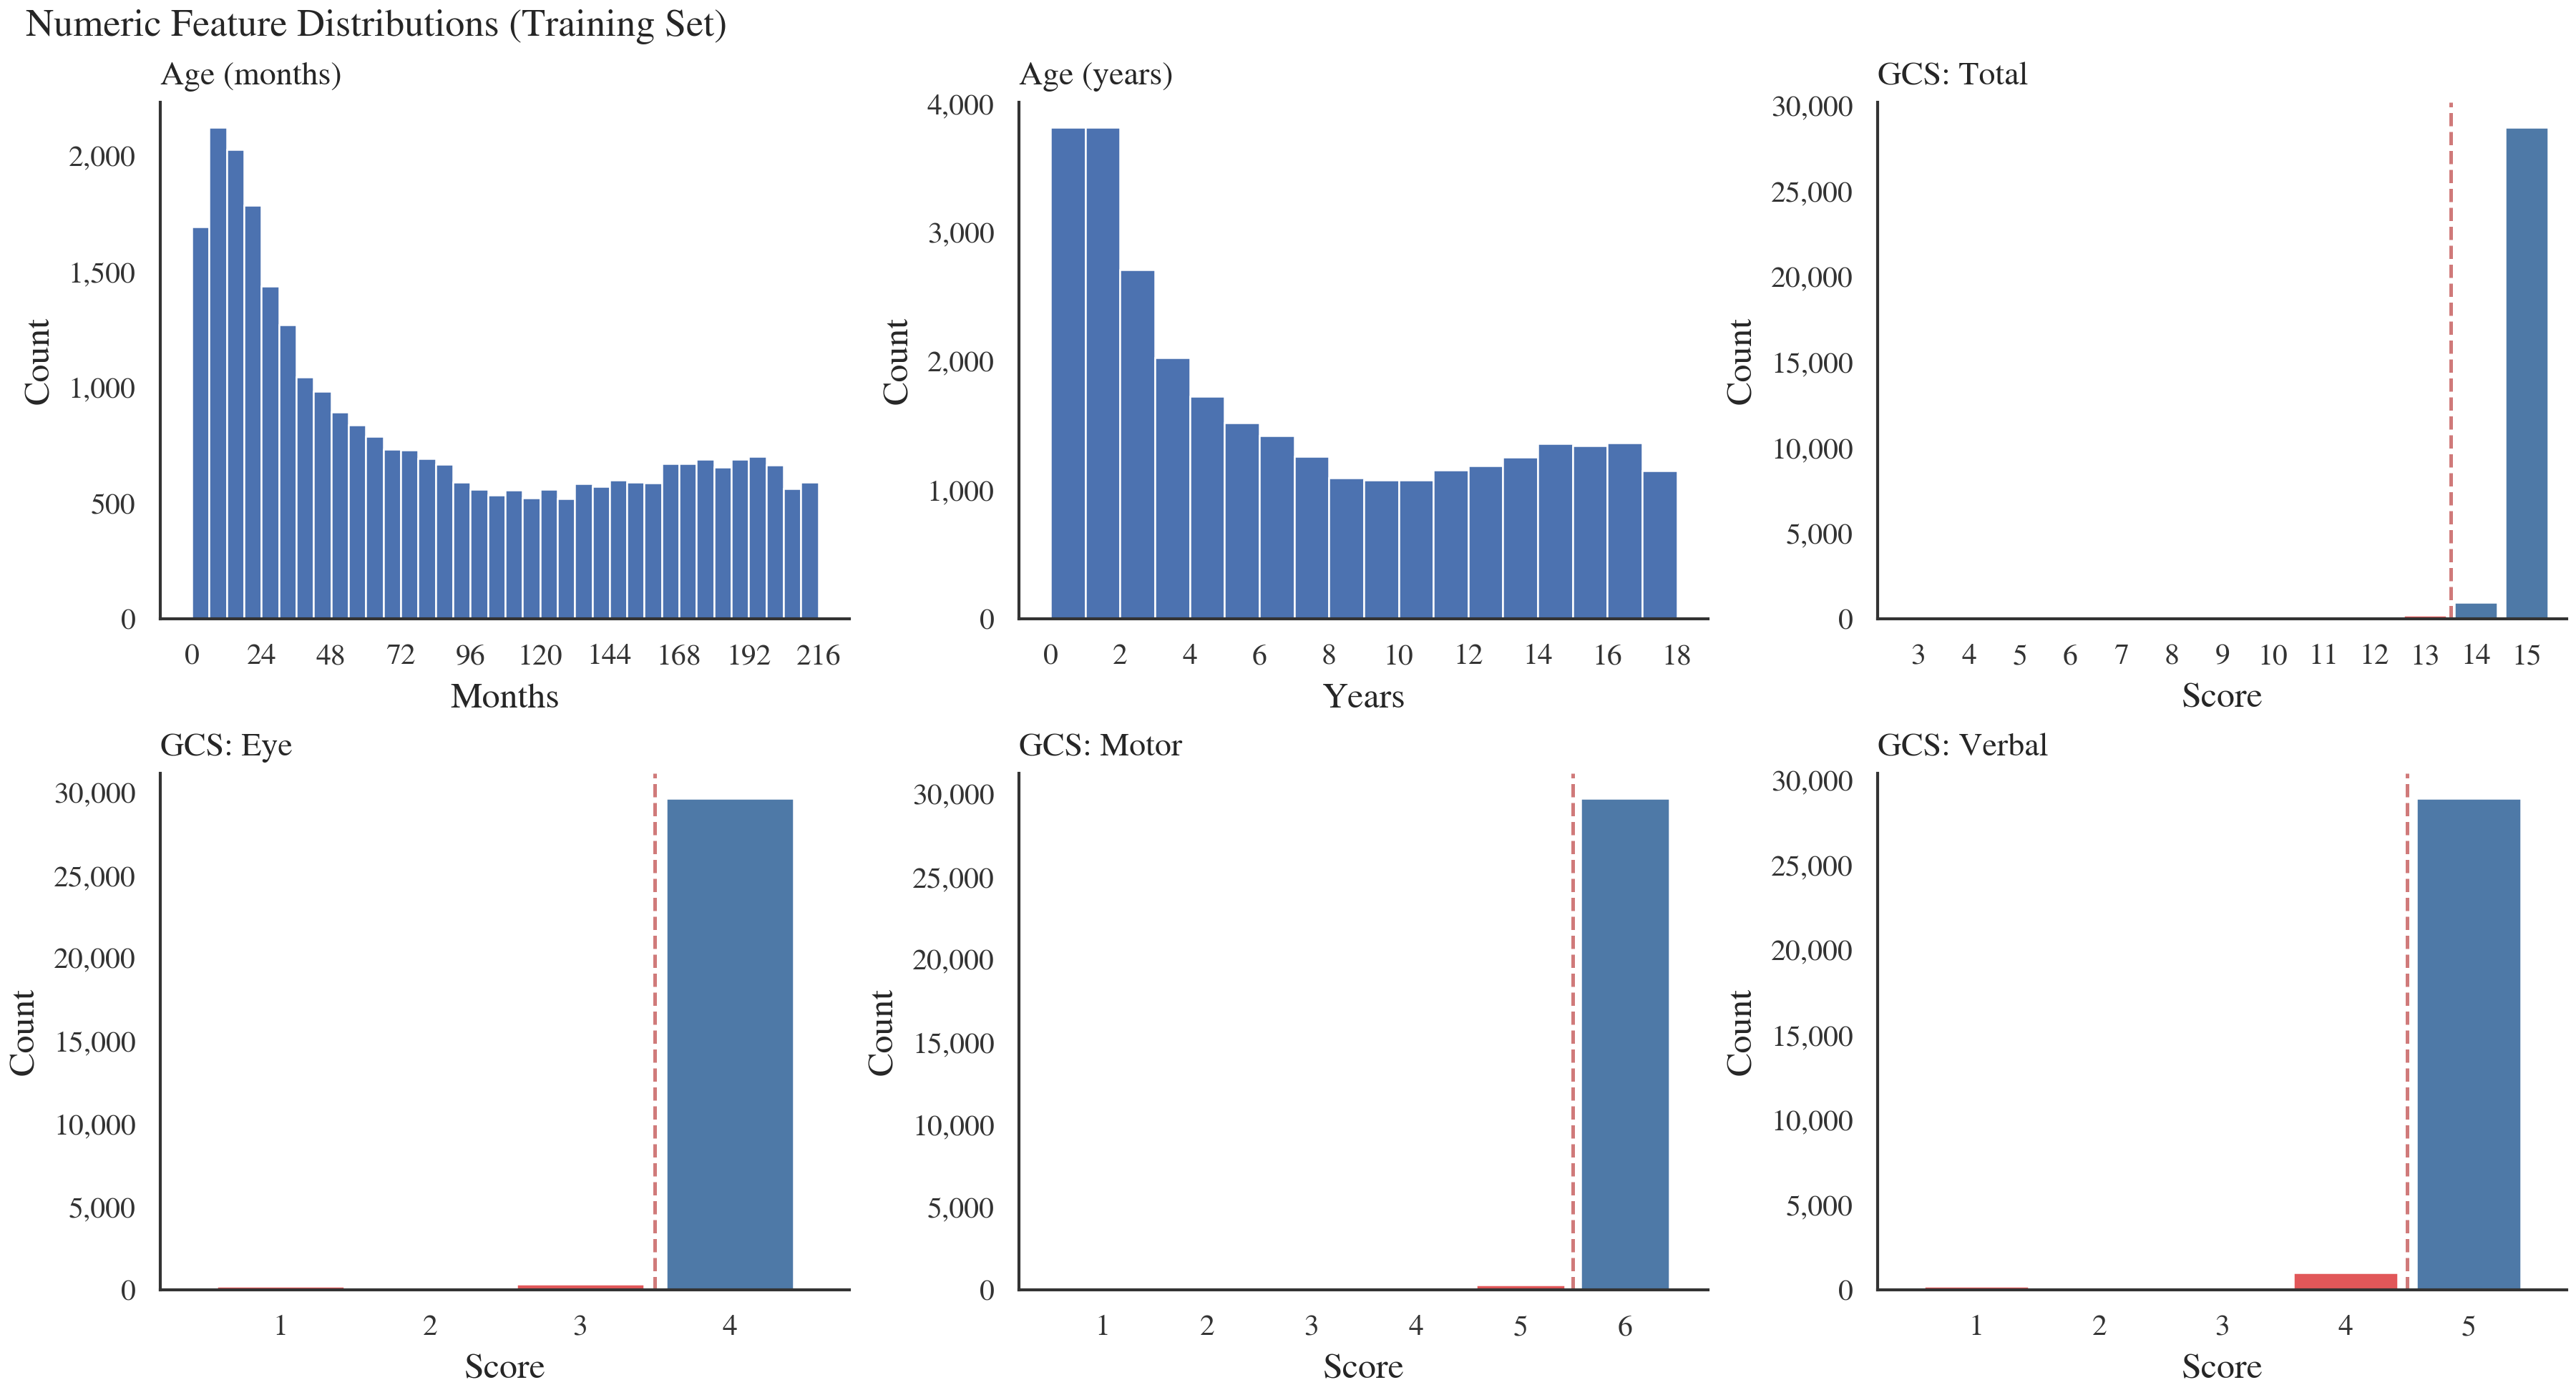
\includegraphics[
    width=1\textwidth,
    height=0.40\textheight,
    keepaspectratio
]{../figs/numeric_feature_distributions.png}
    \caption{Distribution of key numeric variables in the training set, including age and
Glasgow Coma Scale (GCS) components. Most patients present with near-normal
GCS scores (14–15), reflecting the predominance of mild head trauma in the
PECARN cohort.}
    \label{fig:numeric-dists}
\end{figure}

\subsubsection*{Why age matters?}

We have seen the threshold of age 2 along the way, so how is it related with CT utilization and our target ciTBI risk? I use 2 years as the threshold to start my exploration. It turns out young child have a lower CT utilization of 32.3\% compared with group aged at 2 and older, which is 38.2\%. The difference between observed ciTBI risk is not much bigger (1.4\% and 1.9\% respectively). What can we infer from the CT utilization difference across age groups is becomes my first finding in the next section.


\begin{figure}[htbp]
\centering
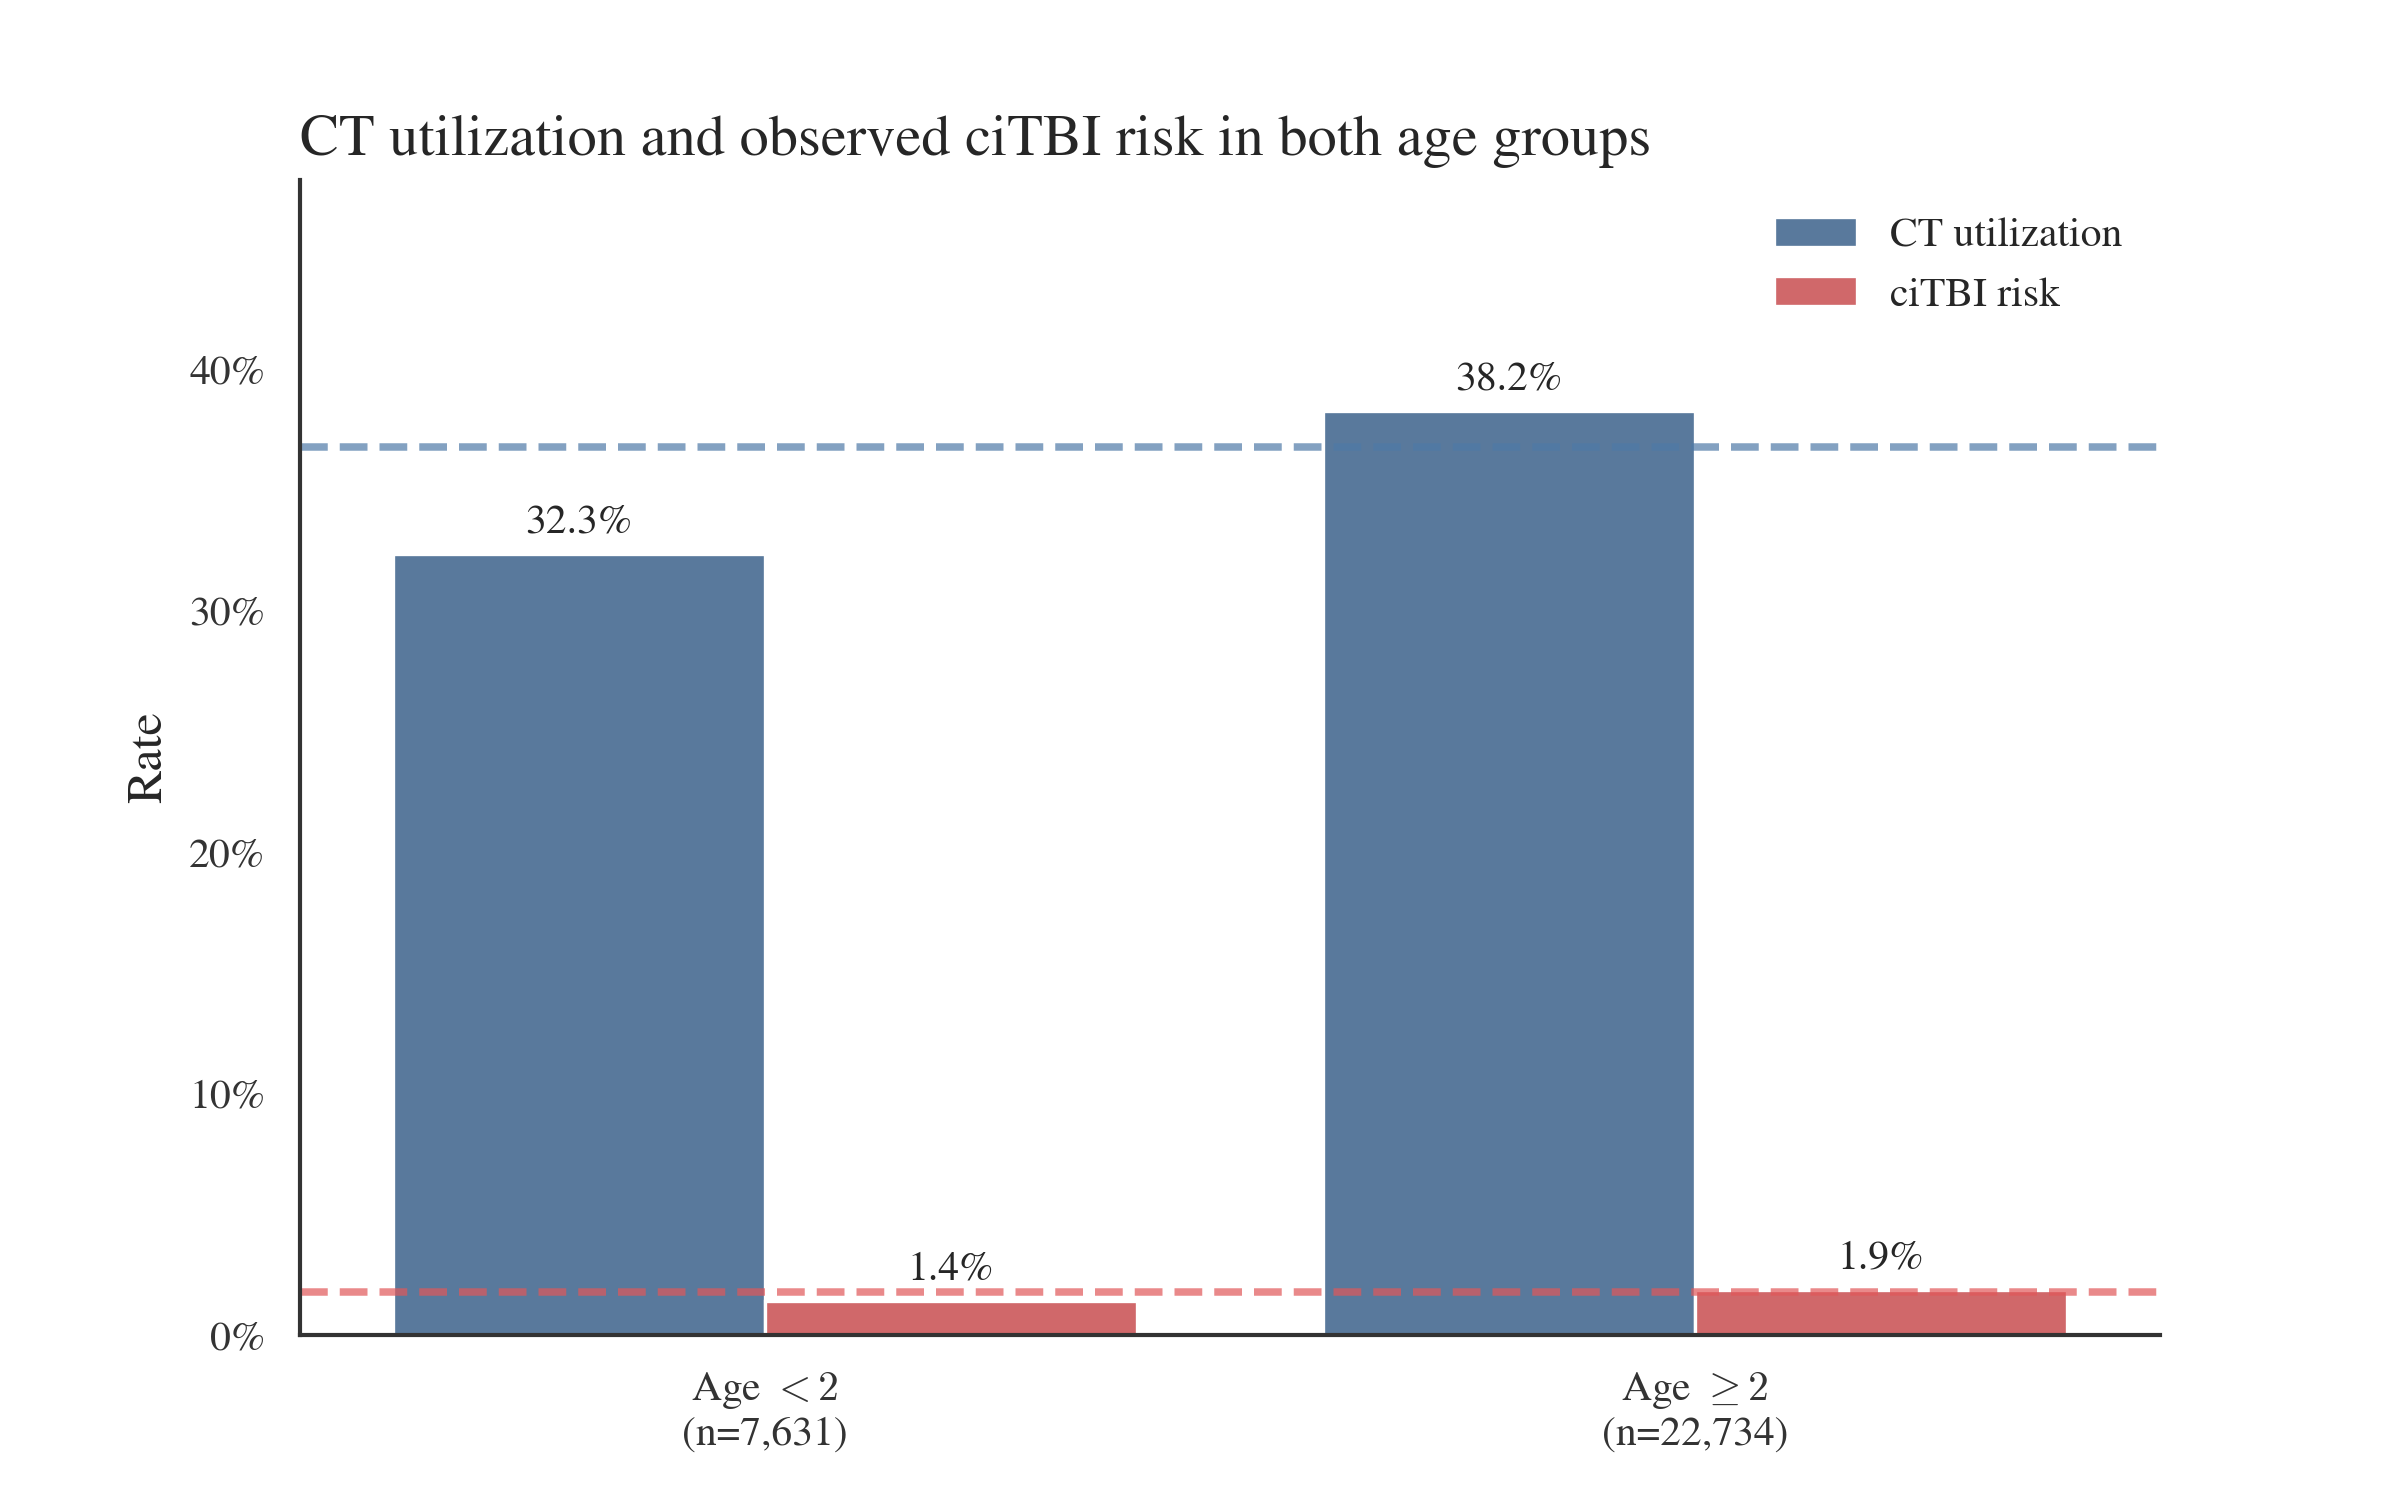
\includegraphics[
    width=1\textwidth,
    height=0.30\textheight,
    keepaspectratio
]{../figs/ct_utilization_and_risk_by_ageTwoplus.png}
\caption{Comparison between CT utilization and observed clinically important traumatic
brain injury (ciTBI) risk across age groups. CT imaging rates substantially
exceed observed risk in both groups, with higher utilization among children
aged $\geq$2 years, illustrating a persistent imaging–risk gap.}
\label{fig:ct-use-age-group}
\end{figure}

\subsubsection*{How do CT decision drivers change with age?}

We next investigate what drives CT assignment and whether these drivers
vary systematically across age groups. Figure~\ref{fig:age_driven_patterns}
shows two complementary perspectives.

Among infants, \textbf{young age itself} is the dominant justification
for imaging, accounting for 63\% of CT assignments. As children grow older,
clinical reasoning shifts toward objective risk indicators. In particular,
\textbf{mechanism of injury} remains important across all ages, while
\textbf{loss of consciousness} becomes increasingly influential after age 10.

This shift aligns with underlying injury epidemiology. Younger children
are primarily injured by falls, whereas adolescents show increasing
contributions from assault and motor vehicle collisions.

\begin{figure}[htbp]
\centering

\begin{subfigure}{0.8\textwidth}
    \centering
    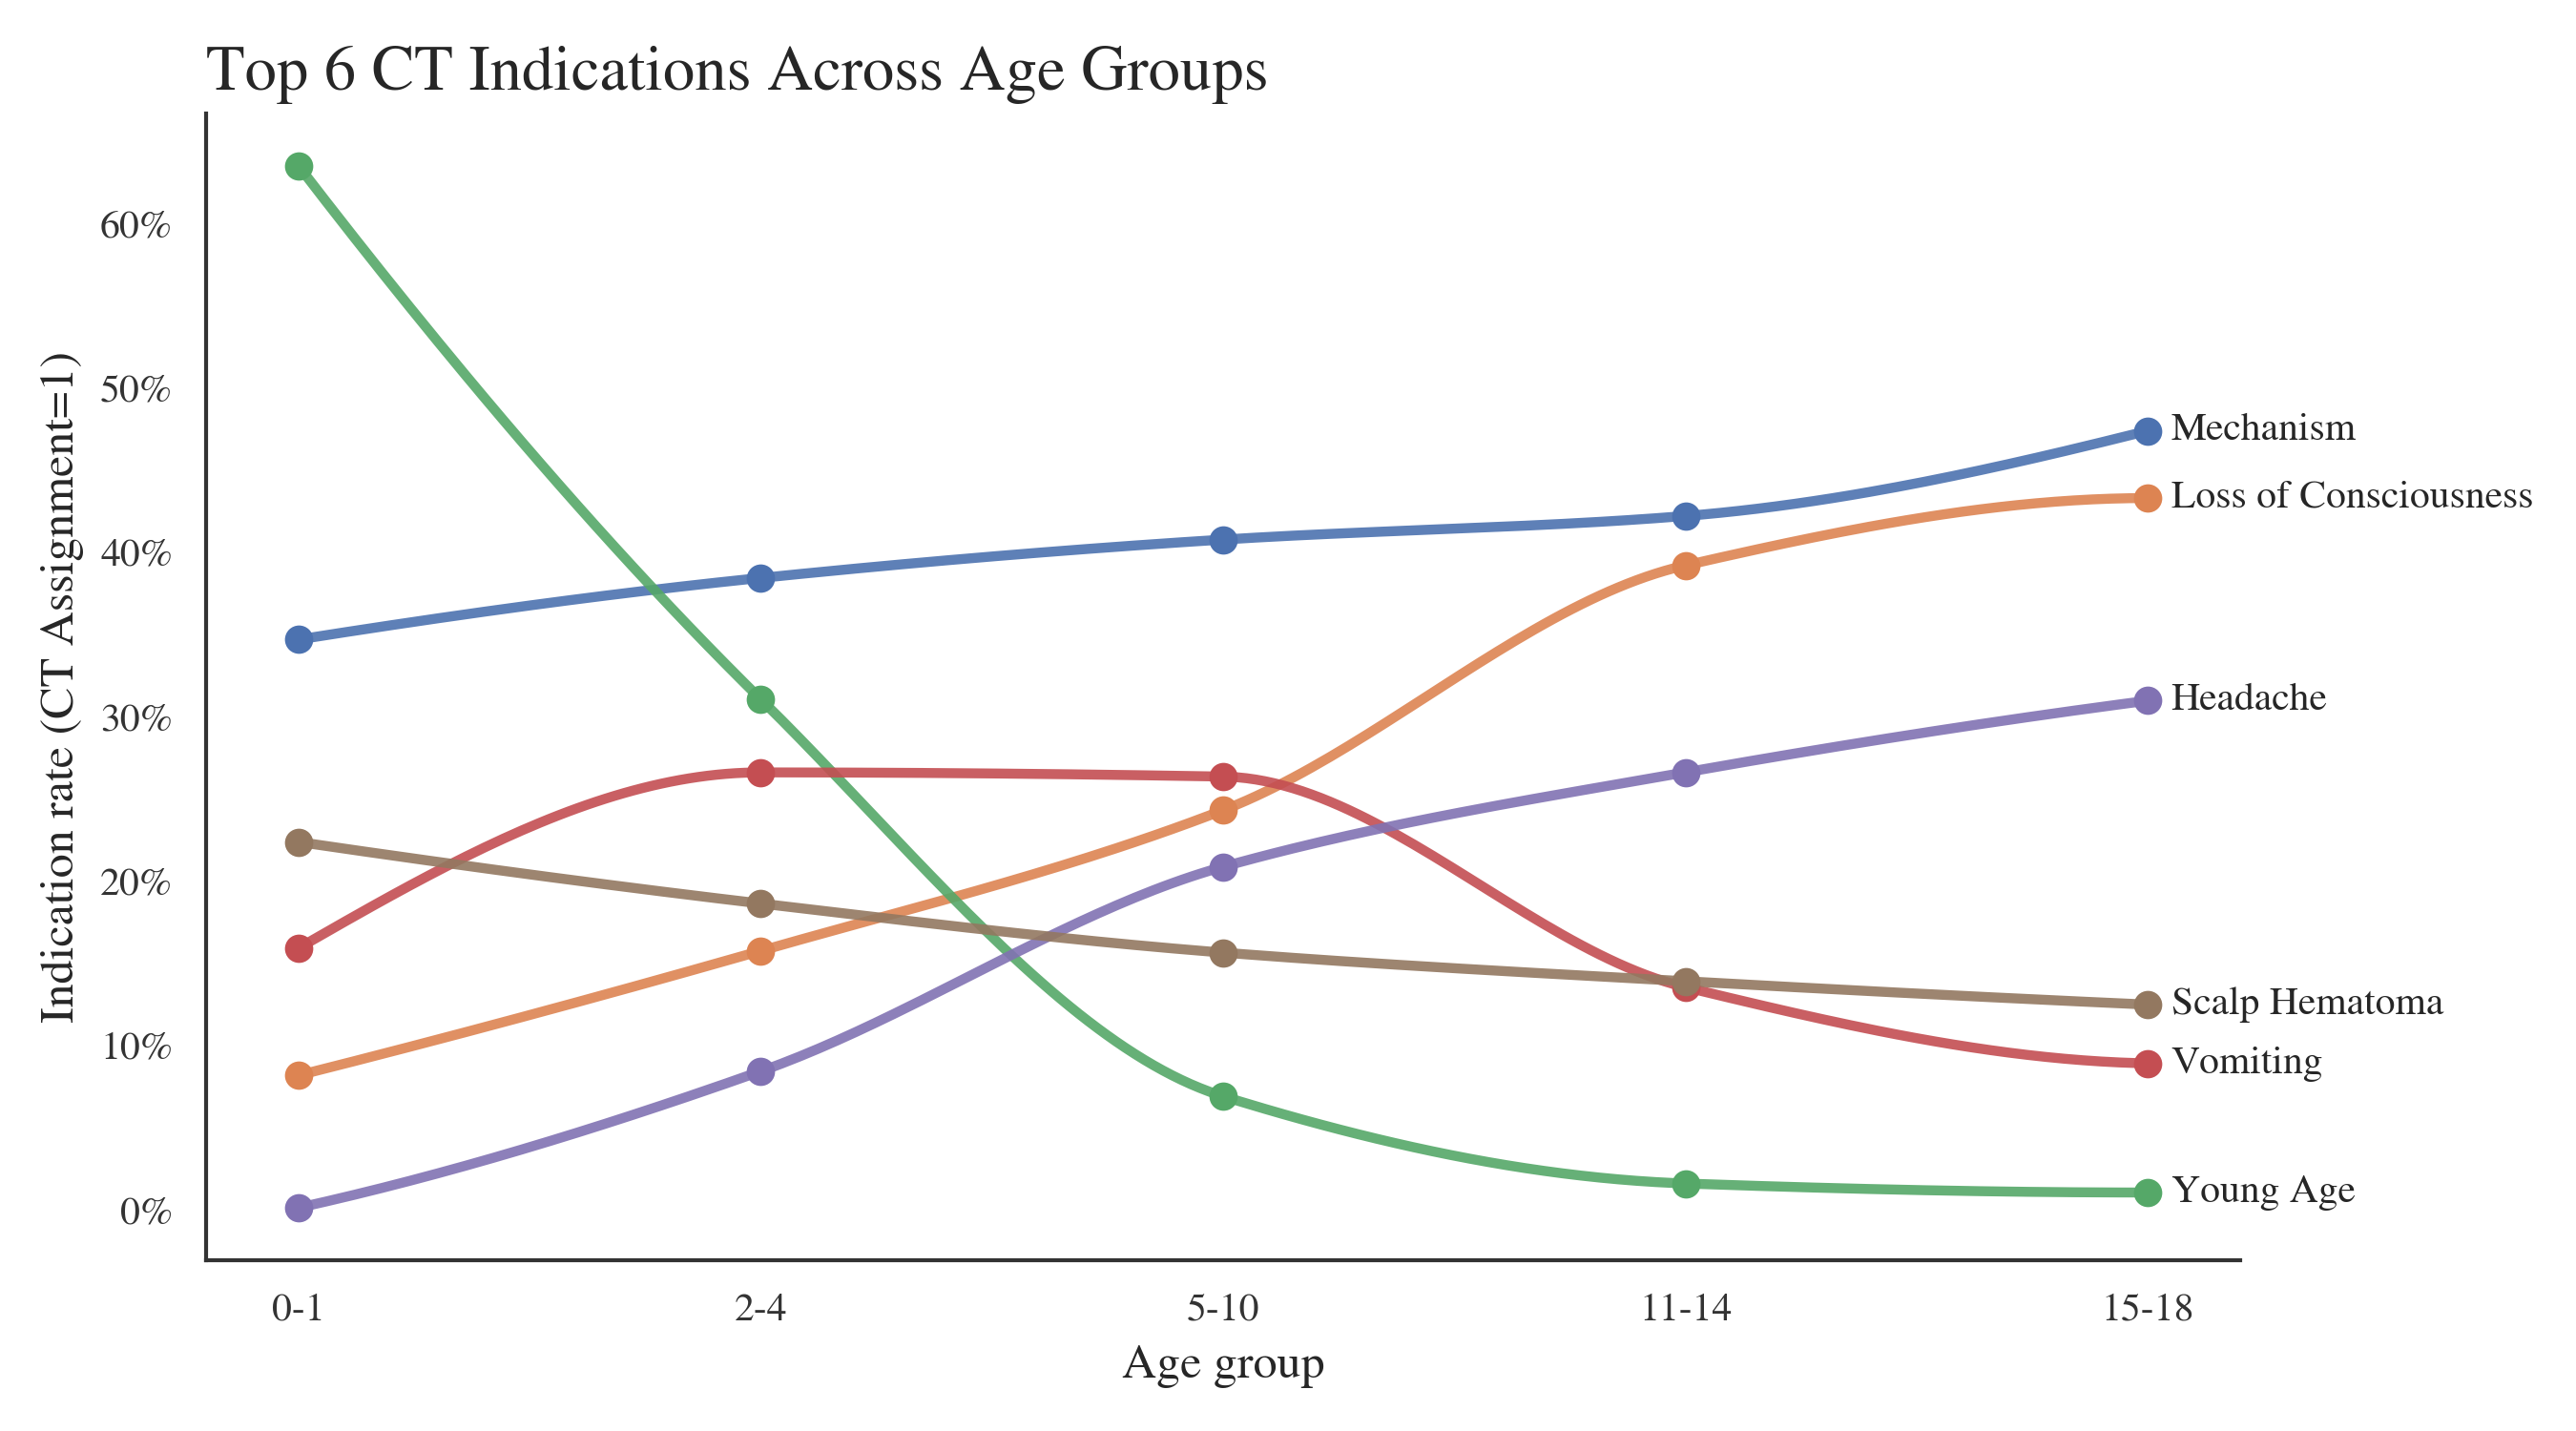
\includegraphics[width=\linewidth]{../figs/ct_indications_by_age.png}
    \caption{CT indications}
\end{subfigure}

\vspace{0.5em}

\begin{subfigure}{0.8\textwidth}
    \centering
    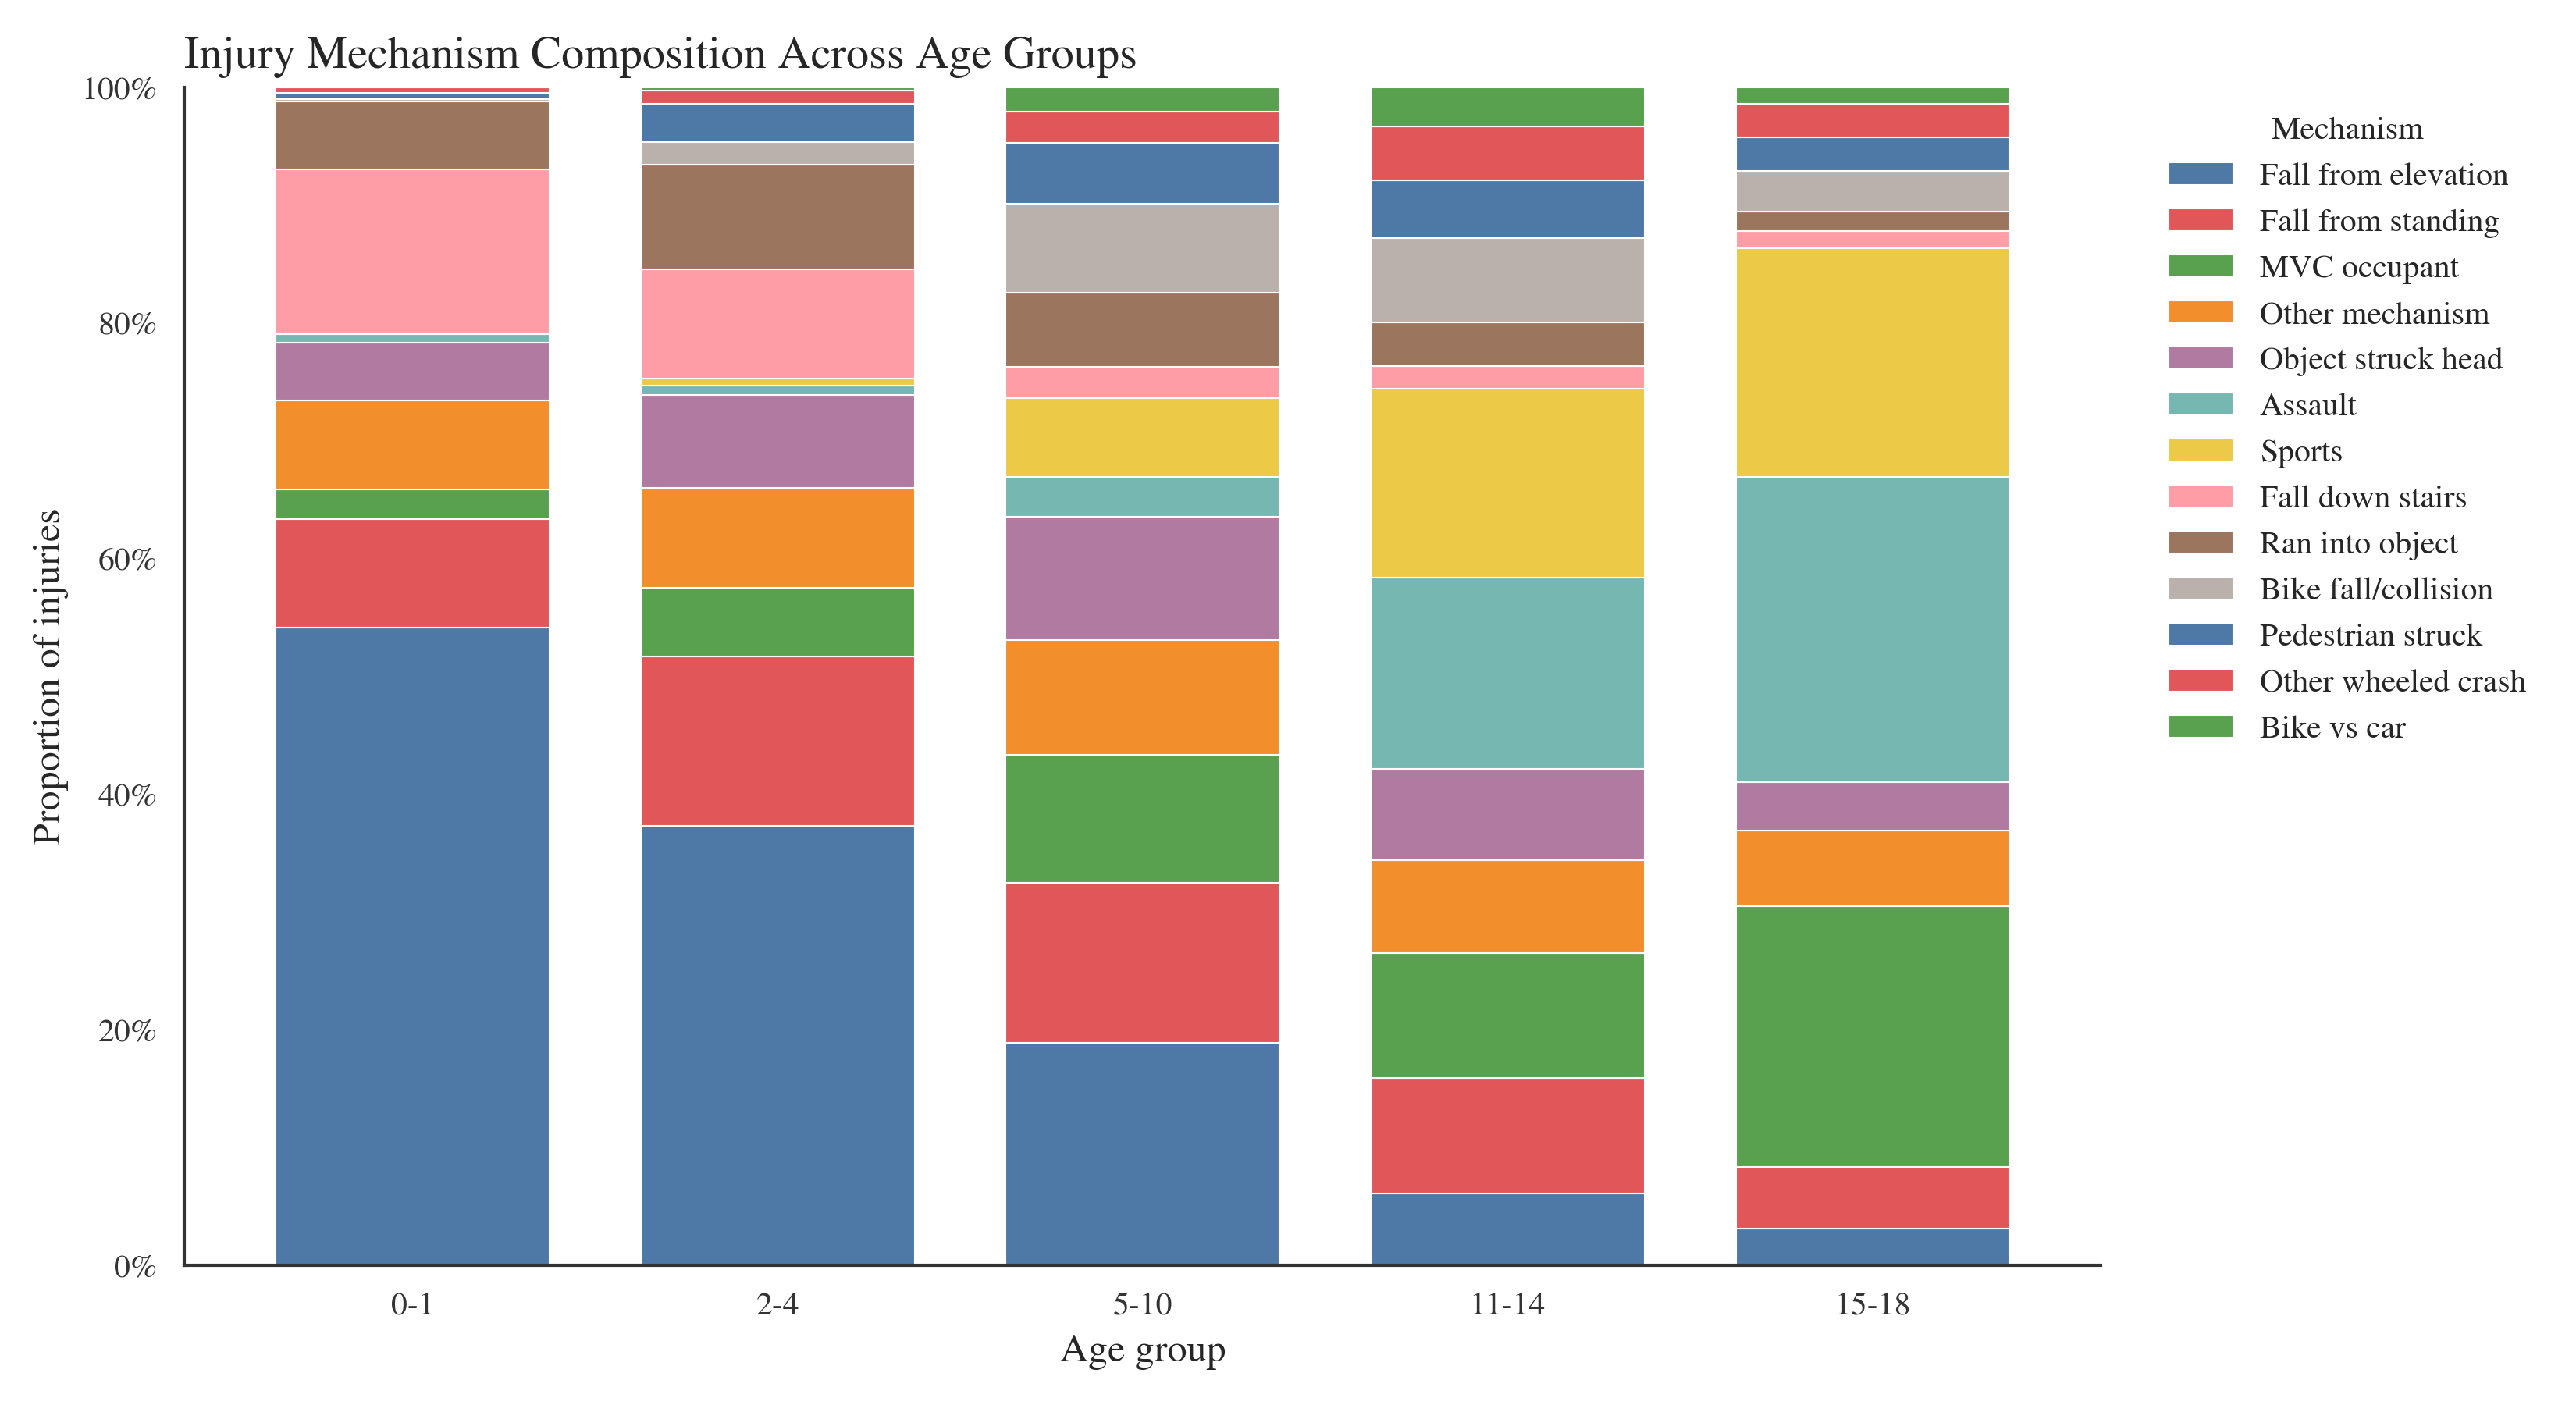
\includegraphics[width=\linewidth]{../figs/injury_mechanism_by_age.png}
    \caption{Injury mechanisms}
\end{subfigure}

\caption{
Age-dependent shifts in CT decision drivers.
\textbf{(a)} The clinical indications motivating CT imaging change with age:
young age dominates in infants, while symptoms such as loss of consciousness
and headache become increasingly influential in older children.
\textbf{(b)} Injury mechanisms also evolve across age groups, shifting from
falls in younger patients toward sports- and vehicle-related injuries in
adolescents.
}
\label{fig:age_driven_patterns}
\end{figure}

\subsubsection*{Other explorations}
Other explorations around new predictors outside the orinial CDR are carried out. Core conclusion is left as my third finding. I would give a brief description about what I have done here. 
\begin{itemize}
\item \textbf{Is there any single predictor useful outside of the CDR?} I first look at the univariate relationship between each predictor and the outcome variable. I find that there are some predictors that are not included in the final CDR but are still statistically significant; I take into account the missingness of the predictors. For prediction, the features we have except GCS are all categorical variables. I use chi-square test to check the association and information value to check the predictability. I do find some meaningful predictors outside of the CDR, like \texttt{NeuroD} (Neurological deficit (other than mental status)?) and \texttt{Seiz} (Post-traumatic seizure?)
\item \textbf{Can any interaction have a better predictiability?} I have inspected the correlation of varaible pairs. To see whether some symptoms usually happen together, their combination may be more predictive than the single, which means the synergy effect.
\end{itemize}


\section{Findings}\label{findings}


\subsection{First finding: CT Utilization is Non-monotonic across Age}\label{first-finding}


In the original clinical decision rule (CDR), patients are divided into two groups: age $<2$ and age $\ge 2$. One important reason for this distinction is that several decisive clinical symptoms are difficult to assess reliably in very young children. For example, symptoms such as amnesia depend on verbal communication, which may not yet be fully developed in infants. Consequently, younger children may be evaluated more conservatively in clinical practice.

When examining CT utilization across finer age strata, a similar pattern emerges. We observe a clear \textbf{turning point} during infancy: children younger than one year exhibit relatively high CT utilization. After age one, CT usage increases gradually with age, suggesting that older children are progressively more likely to receive CT imaging during evaluation.

To better understand this pattern, we examine the clinical indication variable \texttt{IndAge}, which records whether “young age” was explicitly documented as a reason for ordering a CT scan. As shown in the right panel of Figure~\ref{fig:Age CT story}, approximately 73\% of infants (age 0) who received imaging had young age cited as a primary justification. This proportion declines steadily with increasing age, indicating that age itself plays a major role in early imaging decisions.

Together, these results suggest that CT utilization is not driven solely by observed injury risk but also by \textbf{age-dependent} clinical uncertainty, especially in infants.
\begin{figure}[h]
    \centering
    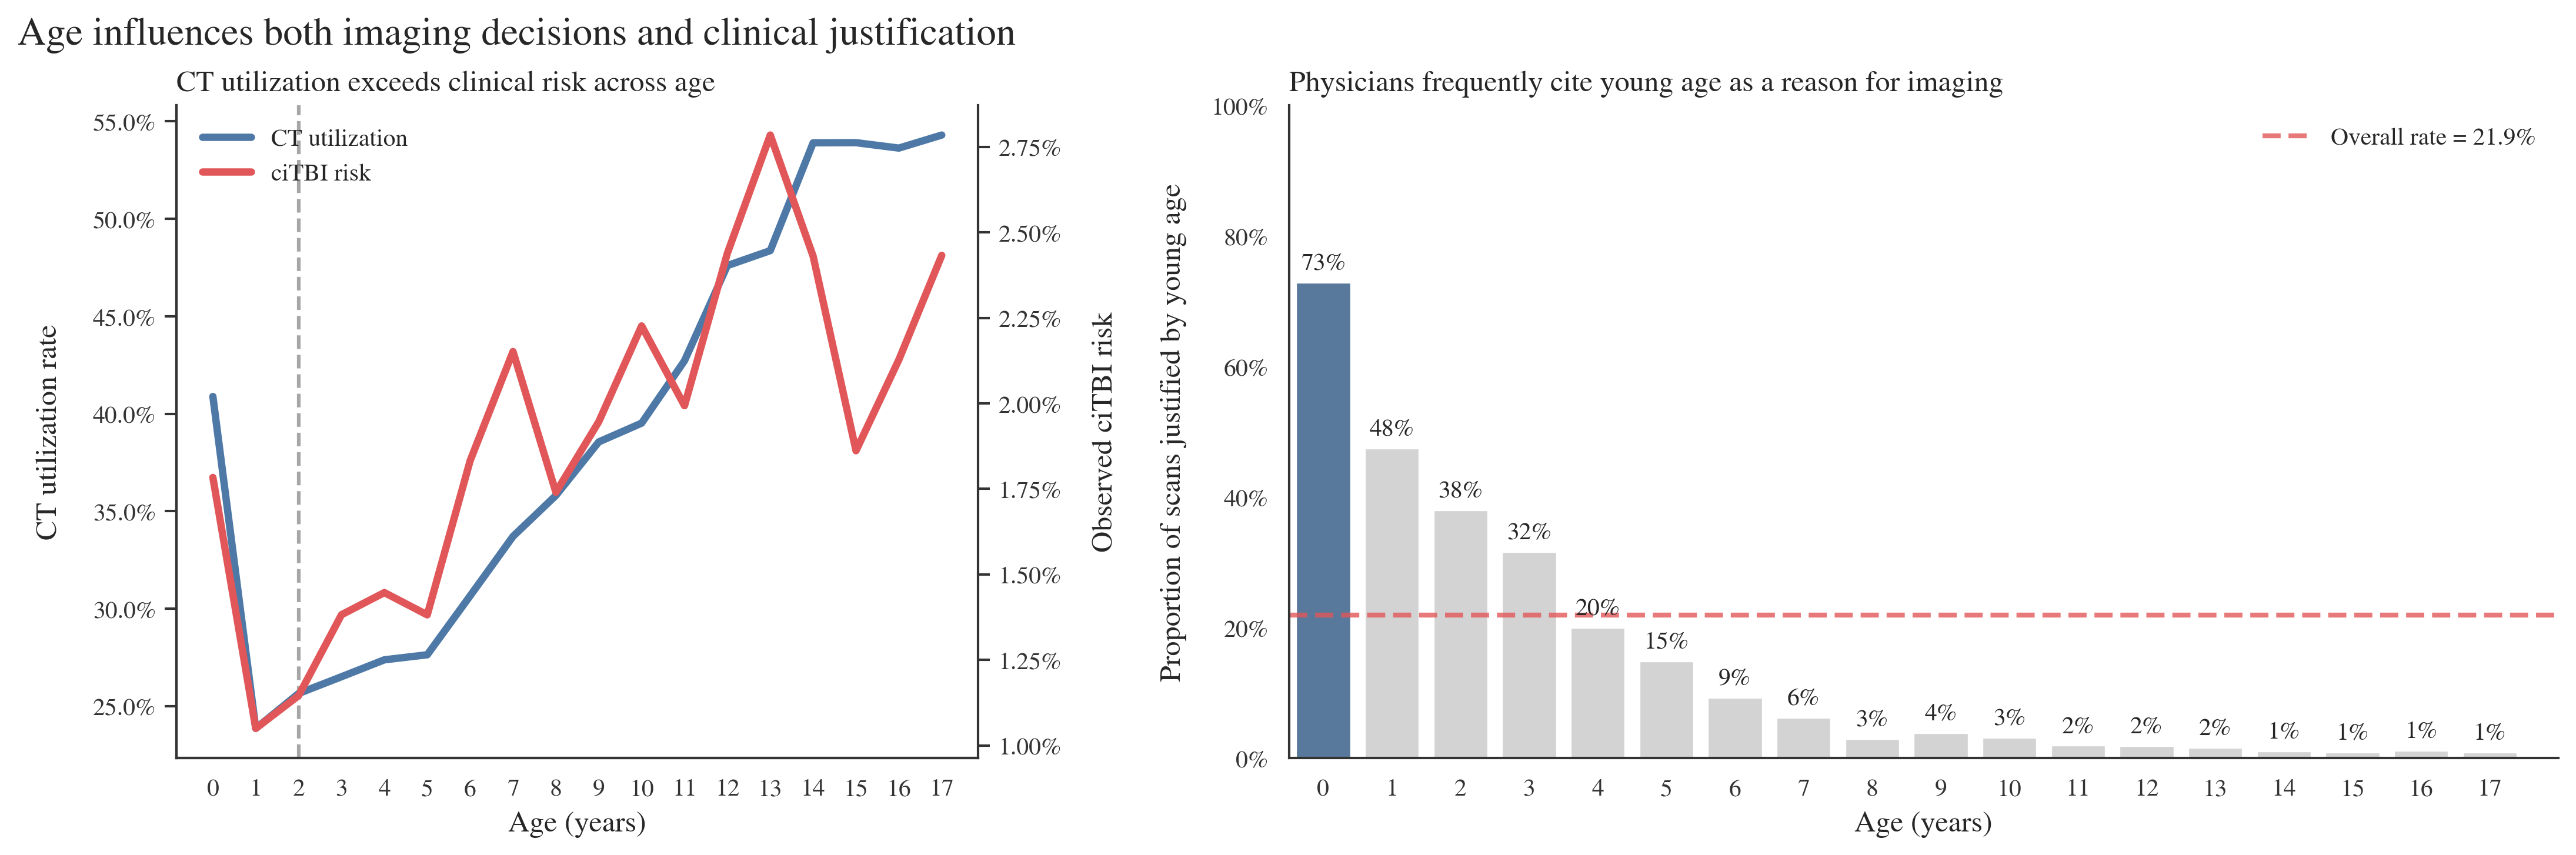
\includegraphics[width=1\textwidth]{../figs/age_ct_story.png}
    \caption{Age influences both CT utilization and clinical justification.
\textbf{Left:} CT use increases with age and consistently exceeds observed
ciTBI risk; the dashed line marks the 2-year clinical threshold.
\textbf{Right:} Young age is frequently cited as a reason for imaging,
especially in infants, with justification rates declining steadily with age.}
    \label{fig:Age CT story} 
\end{figure}

\subsection{Second finding: Over-scanning Varies across Mechnism}\label{second-finding}

We define the \textbf{over-scan} gap as the difference between the CT utilization rate and the observed ciTBI risk. A larger gap reflects more conservative imaging behavior relative to outcome risk.

Our analysis shows that imaging decisions differ substantially across injury mechanisms. High-energy mechanisms — such as pedestrian struck by a vehicle or bicycle-automobile collisions — are associated with consistently larger over-scan gaps. In these scenarios, physicians appear to favor precautionary imaging even when the observed outcome risk alone would not fully justify the imaging rate.

This pattern suggests a form of \textbf{risk-averse clinical behavior}, where mechanisms perceived as severe trigger additional imaging independent of measured risk.

In contrast, lower-energy mechanisms (e.g., running into an object or object striking the head) exhibit smaller gaps across age groups, indicating that imaging decisions more closely align with actual outcome risk.

Overall, clinicians appear to adjust imaging strategies according to perceived mechanism severity, highlighting the importance of contextual clinical judgment beyond statistical risk estimates.

I mark some grids grey due to tiny group size which will result in unsolid and misleading analysis. 
\begin{figure}[h]
    \centering
    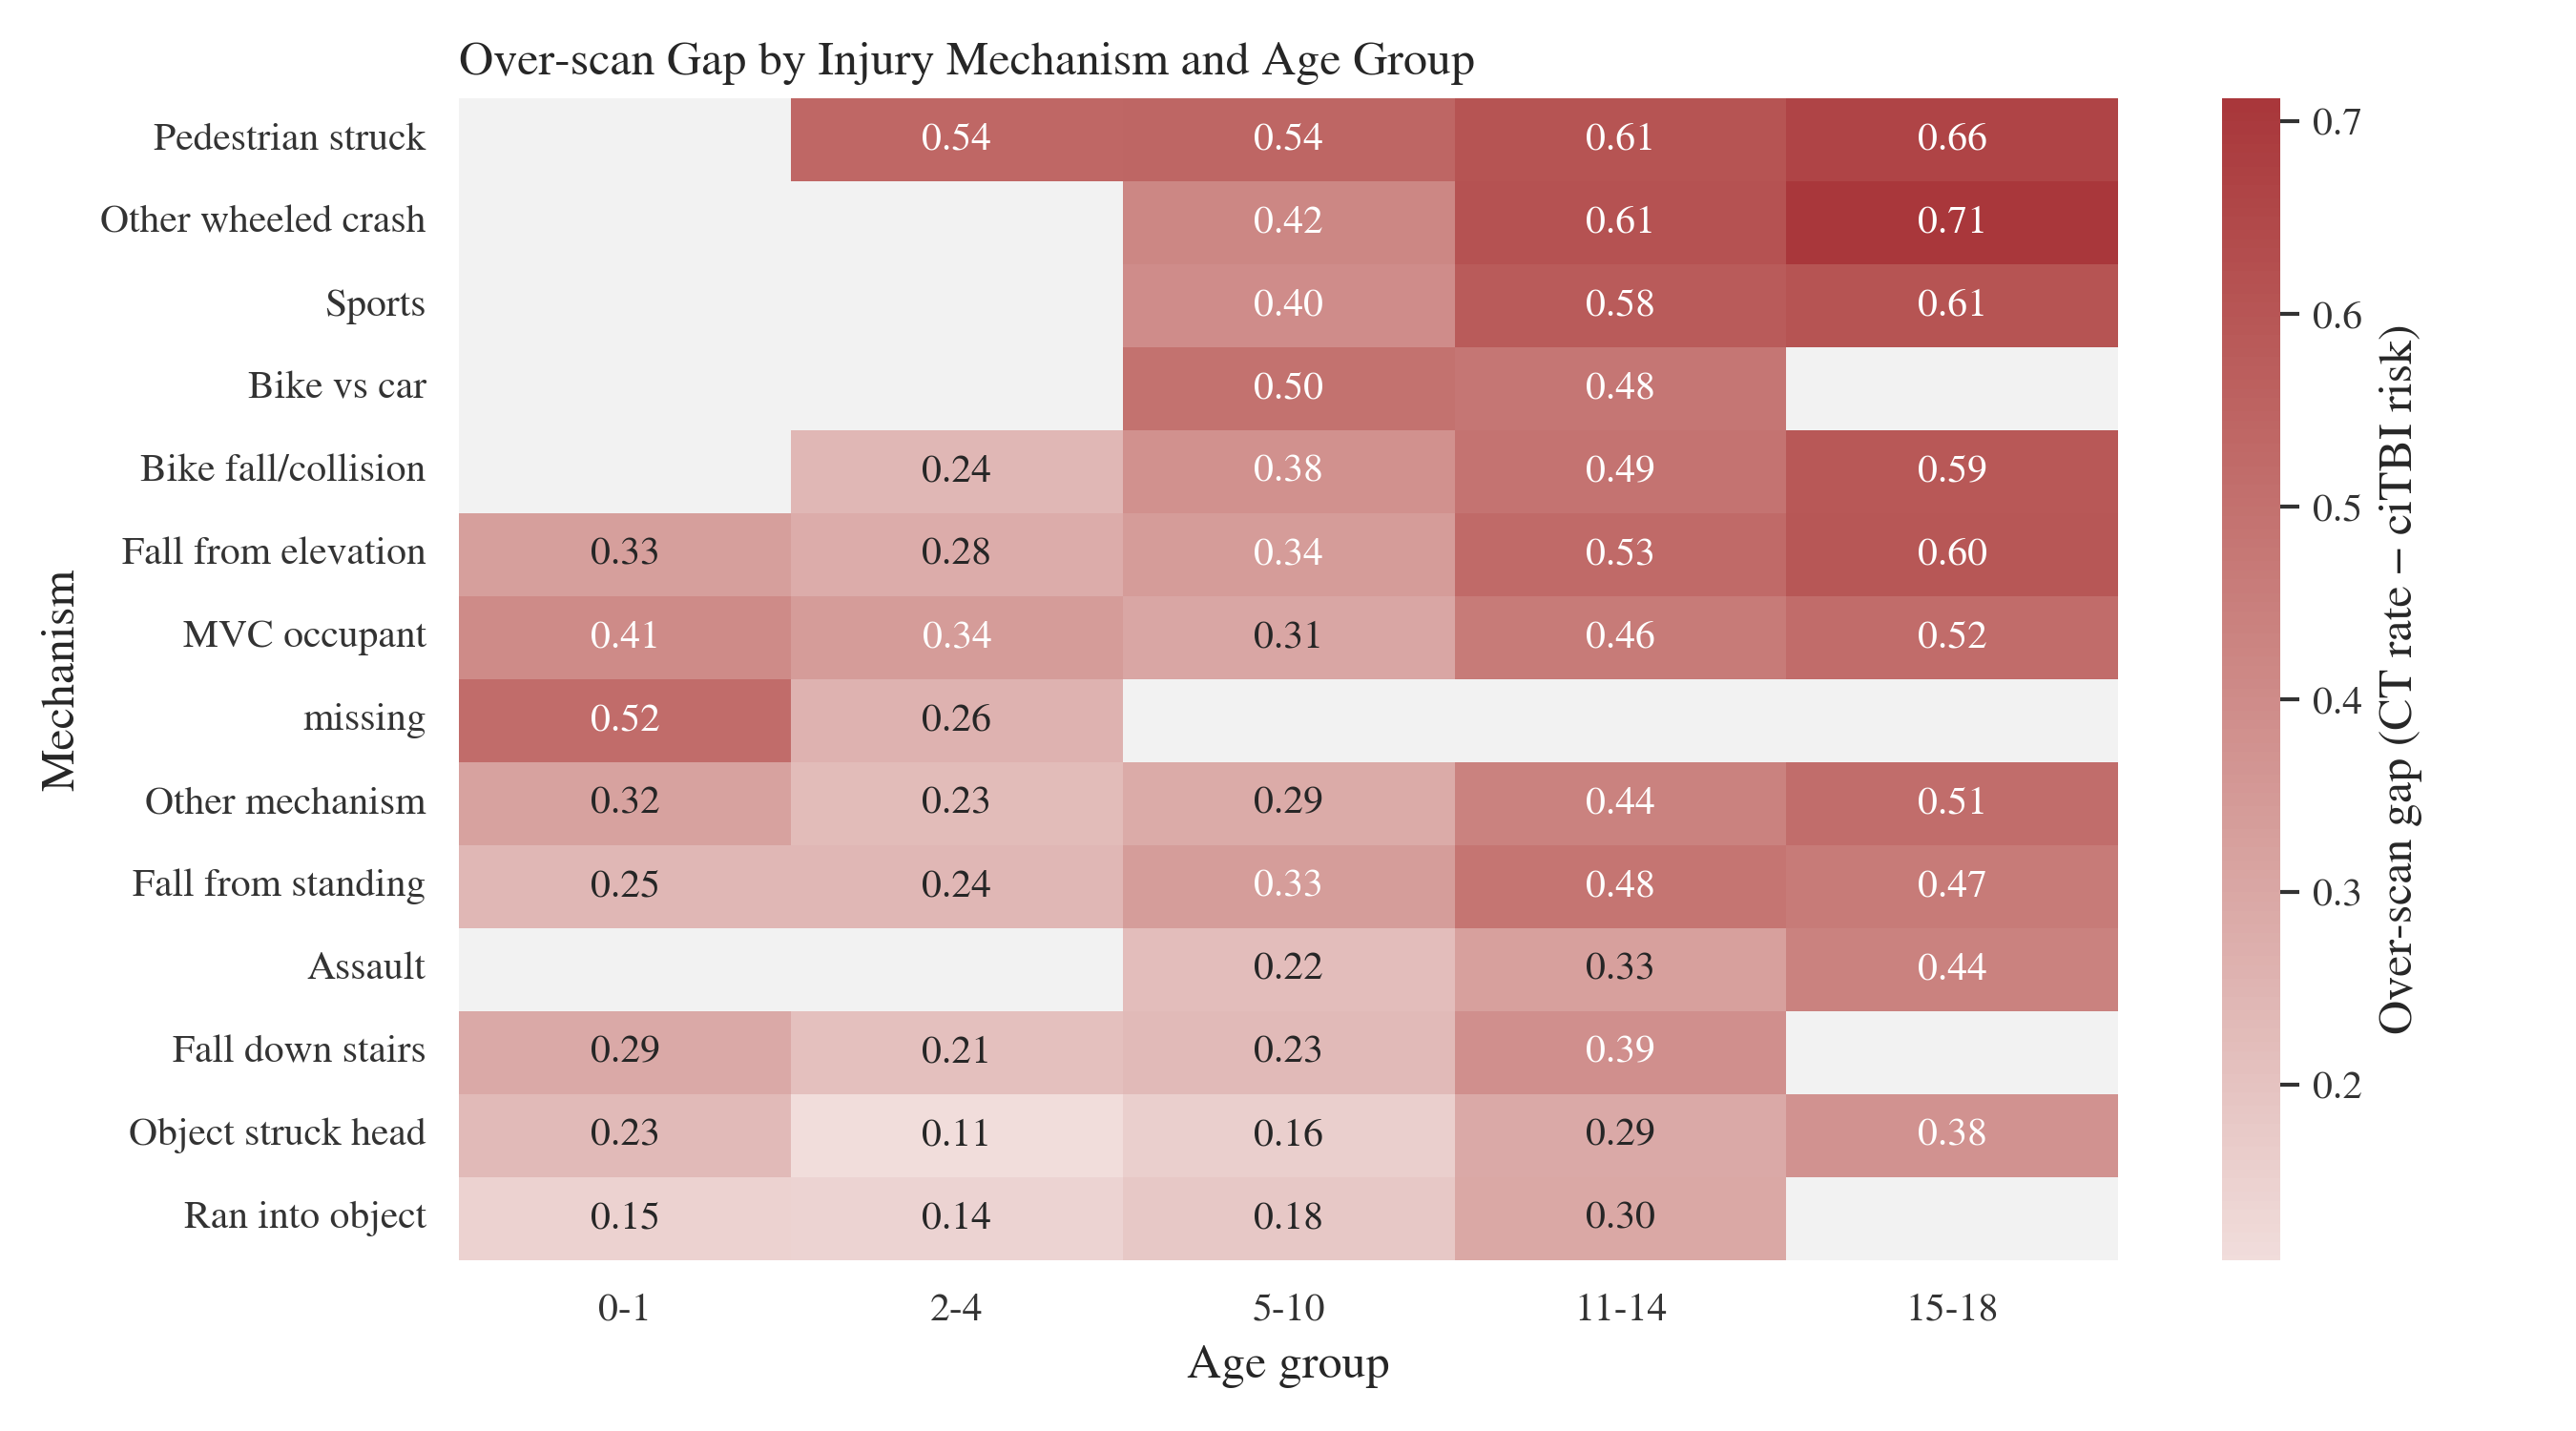
\includegraphics[width=1\textwidth]{../figs/mechanism_heatmap.png}
    \caption{Over-scan gap (CT utilization minus observed ciTBI risk) across injury mechanisms and age groups.
Darker colors indicate larger discrepancies between imaging use and clinical risk.
The gap generally increases with age and varies substantially by mechanism,
suggesting heterogeneous imaging practices beyond risk differences alone.}
    \label{fig:overscan gap by mechanism and age} 
\end{figure}

\subsection{Third finding: Missingness Carries Clinical Signal }\label{third-finding}


Missing clinical variables are often treated purely as data quality issues. However, our analysis suggests that missingness itself may encode clinically meaningful information.

Figure~\ref{fig:missingness effect} shows that patients with missing entries in certain neurological or symptom variables exhibit systematically different ciTBI risks compared with those explicitly recorded as positive or negative. This pattern is consistent across age groups.

A plausible explanation is that missing values frequently arise from the clinical workflow rather than random omission. For example, physicians may skip documenting specific examinations when a patient appears low risk, uncooperative, or clinically stable. As a result, missingness may implicitly reflect physician judgment or examination feasibility.

These findings indicate that missingness should not always be treated as noise; instead, it can function as an informative feature capturing latent clinical decision processes.

Similar strategy has been used in treating the tiny subgroup size issue, which I directly marked as grey. 

\begin{figure}[h]
    \centering
    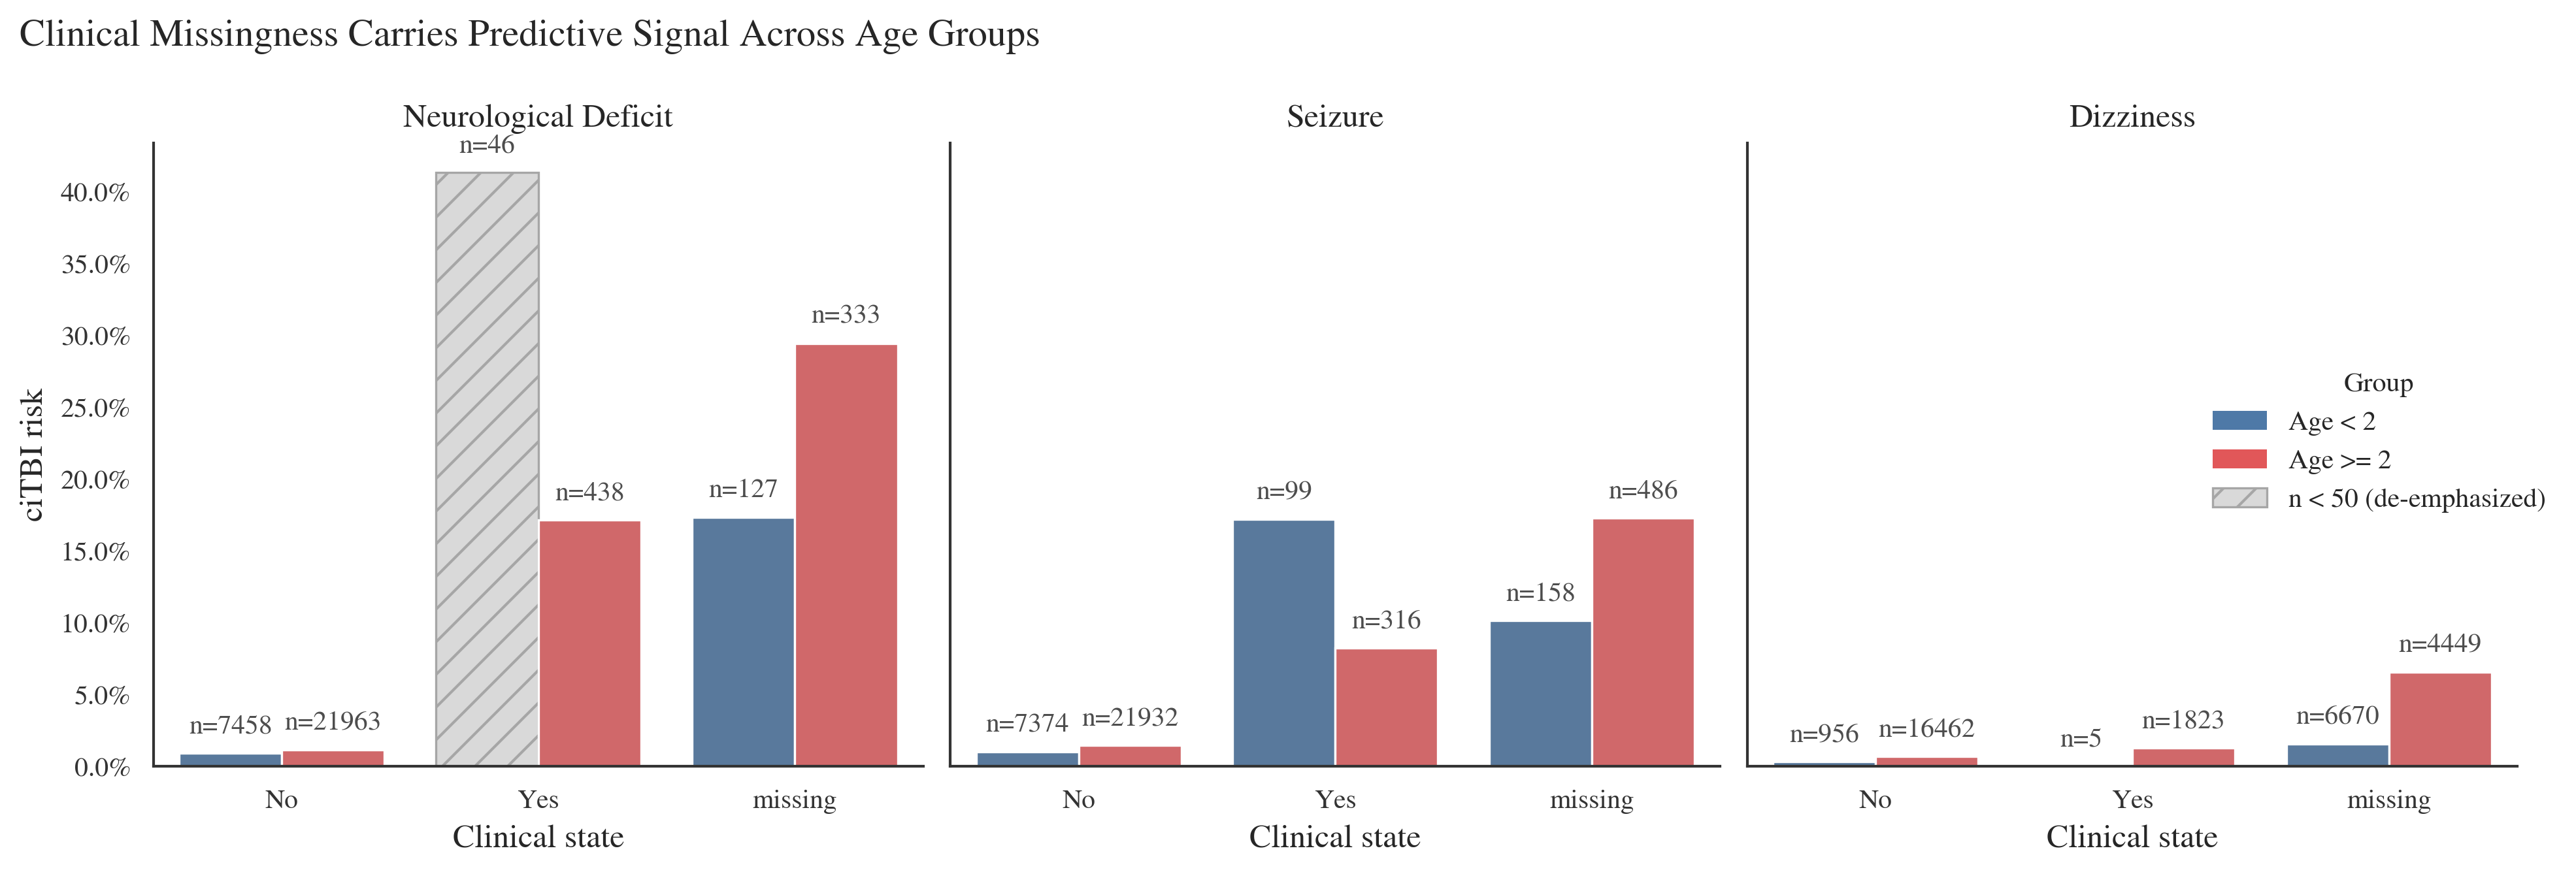
\includegraphics[width=1\textwidth]{../figs/missingness_effect.png}
    \caption{Association between clinical missingness and ciTBI risk across age groups.
Bars show observed risk conditional on clinical state (No, Yes, Missing),
with subgroup sizes annotated above each bar.
De-emphasized bars indicate small sample sizes ($n<50$).
Missingness is associated with systematically different risk levels,
suggesting that unrecorded clinical information may reflect implicit physician judgment.}
    \label{fig:missingness effect} 
\end{figure}

\subsection{Reality Check}\label{reality-check}

During data preprocessing, several judgment calls were made, including the
imputation of GCS component and whether exclude GCS 3-13. To ensure that these decisions did not distort the clinical meaning of the dataset, we performed a reality check by comparing key patterns in the cleaned data with known clinical expectations
and findings reported in the original PECARN study.

\paragraph{Realistic prevalence of clinical outcomes.}
A first sanity check is whether important clinical variables occur at
reasonable frequencies. In the original data, the prevalence of
clinically important traumatic brain injury (ciTBI) was approximately
0.9\% (376 out of 42,412 patients). In our cleaned training dataset, the
overall ciTBI rate is 1.76\%. This slightly higher value is expected because
our dataset includes patients with GCS scores between 3 and 13, whereas the
original analysis focused primarily on children with mild traumatic brain
injury (GCS 14--15). 

To verify this interpretation, we recomputed the risk after excluding
patients with GCS 3--13. The resulting ciTBI prevalence becomes 0.87\%,
which closely matches the published value. This agreement suggests that the
cleaning and inclusion criteria preserve a clinically realistic outcome
distribution.

\paragraph{Clinical monotonicity and age stratification.}
The original study separates preverbal children ($<2$ years) from older
children because younger patients have limited ability to communicate
symptoms and are often managed more conservatively. In our exploratory
analysis, CT utilization and clinical decision patterns show clear age-related
structure consistent with this rationale. Younger children exhibit higher
imaging rates driven by diagnostic uncertainty, while decision drivers shift
toward injury mechanism and neurological symptoms as age increases.
This alignment supports the validity of the preprocessing choices and
reinforces the clinical interpretability of the cleaned dataset.

\paragraph{Clinical meaning of missing data.}
Another important question is whether missing values arise purely from data
quality issues or whether they carry clinical information. Because these data
are collected through physician documentation, missingness may reflect
clinical workflow and judgment rather than randomness. The observed association between missingness patterns and outcome risk therefore suggests that missing values encode latent clinical signal instead of preprocessing artifacts.

\paragraph{Conclusion of reality check.}
Across outcome prevalence, age-related decision patterns, and the behavior of
missing clinical variables, the cleaned dataset remains consistent with
real-world clinical expectations. These findings indicate that the
preprocessing decisions did not introduce major distortions and that the data
pass the reality check required for subsequent modeling and interpretation.

\subsection{Stability Check}\label{stability-check}

To assess robustness, I introduced small random perturbations to selected clinical indication variables and recomputed the age–indication relationship. The overall pattern remains unchanged: young age continues to be a dominant justification for imaging, and the declining trend with increasing age persists. In addition, bootstrap resampling was used to recompute the CT utilization curve across age. The bootstrap curves closely follow the original estimate, preserving the same non-monotonic shape. Together, these results suggest that the finding is stable and not driven by minor data variations or sampling noise.



\begin{figure}[htbp]
    \centering
    \begin{subfigure}[t]{0.48\textwidth}
        \centering
        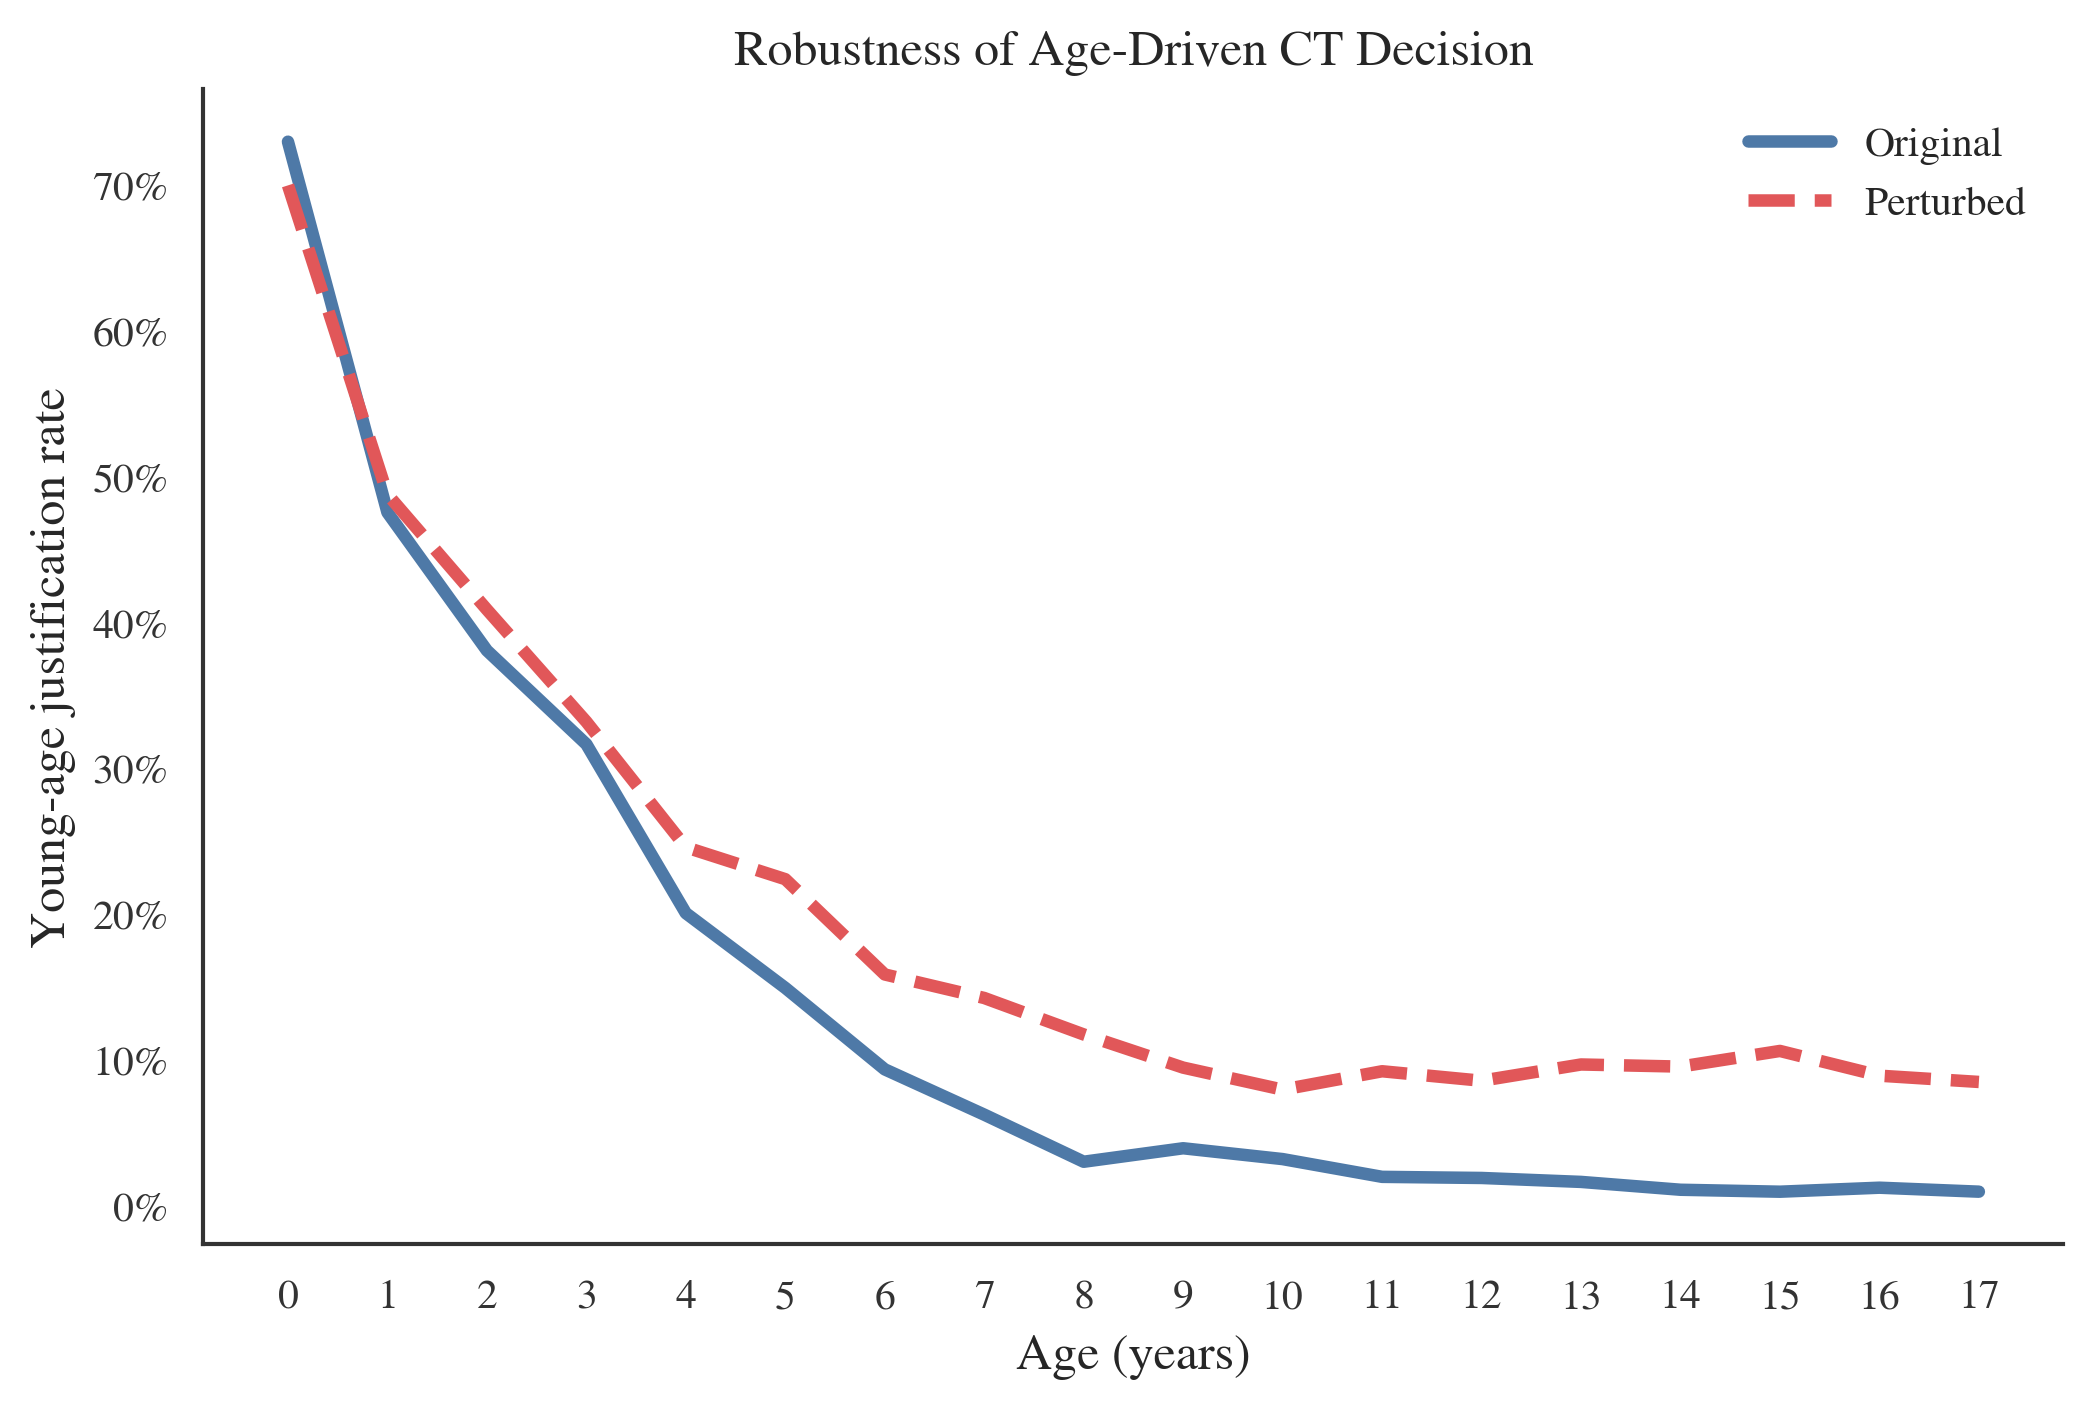
\includegraphics[
            height=0.25\textheight,
            width=\linewidth,
            keepaspectratio
        ]{../figs/age_justification_perturbation.png}
        \caption{Perturbation: age-justification curve is preserved.}
    \end{subfigure}
    \hfill
    \begin{subfigure}[t]{0.48\textwidth}
    \centering
    \raisebox{1ex}{
        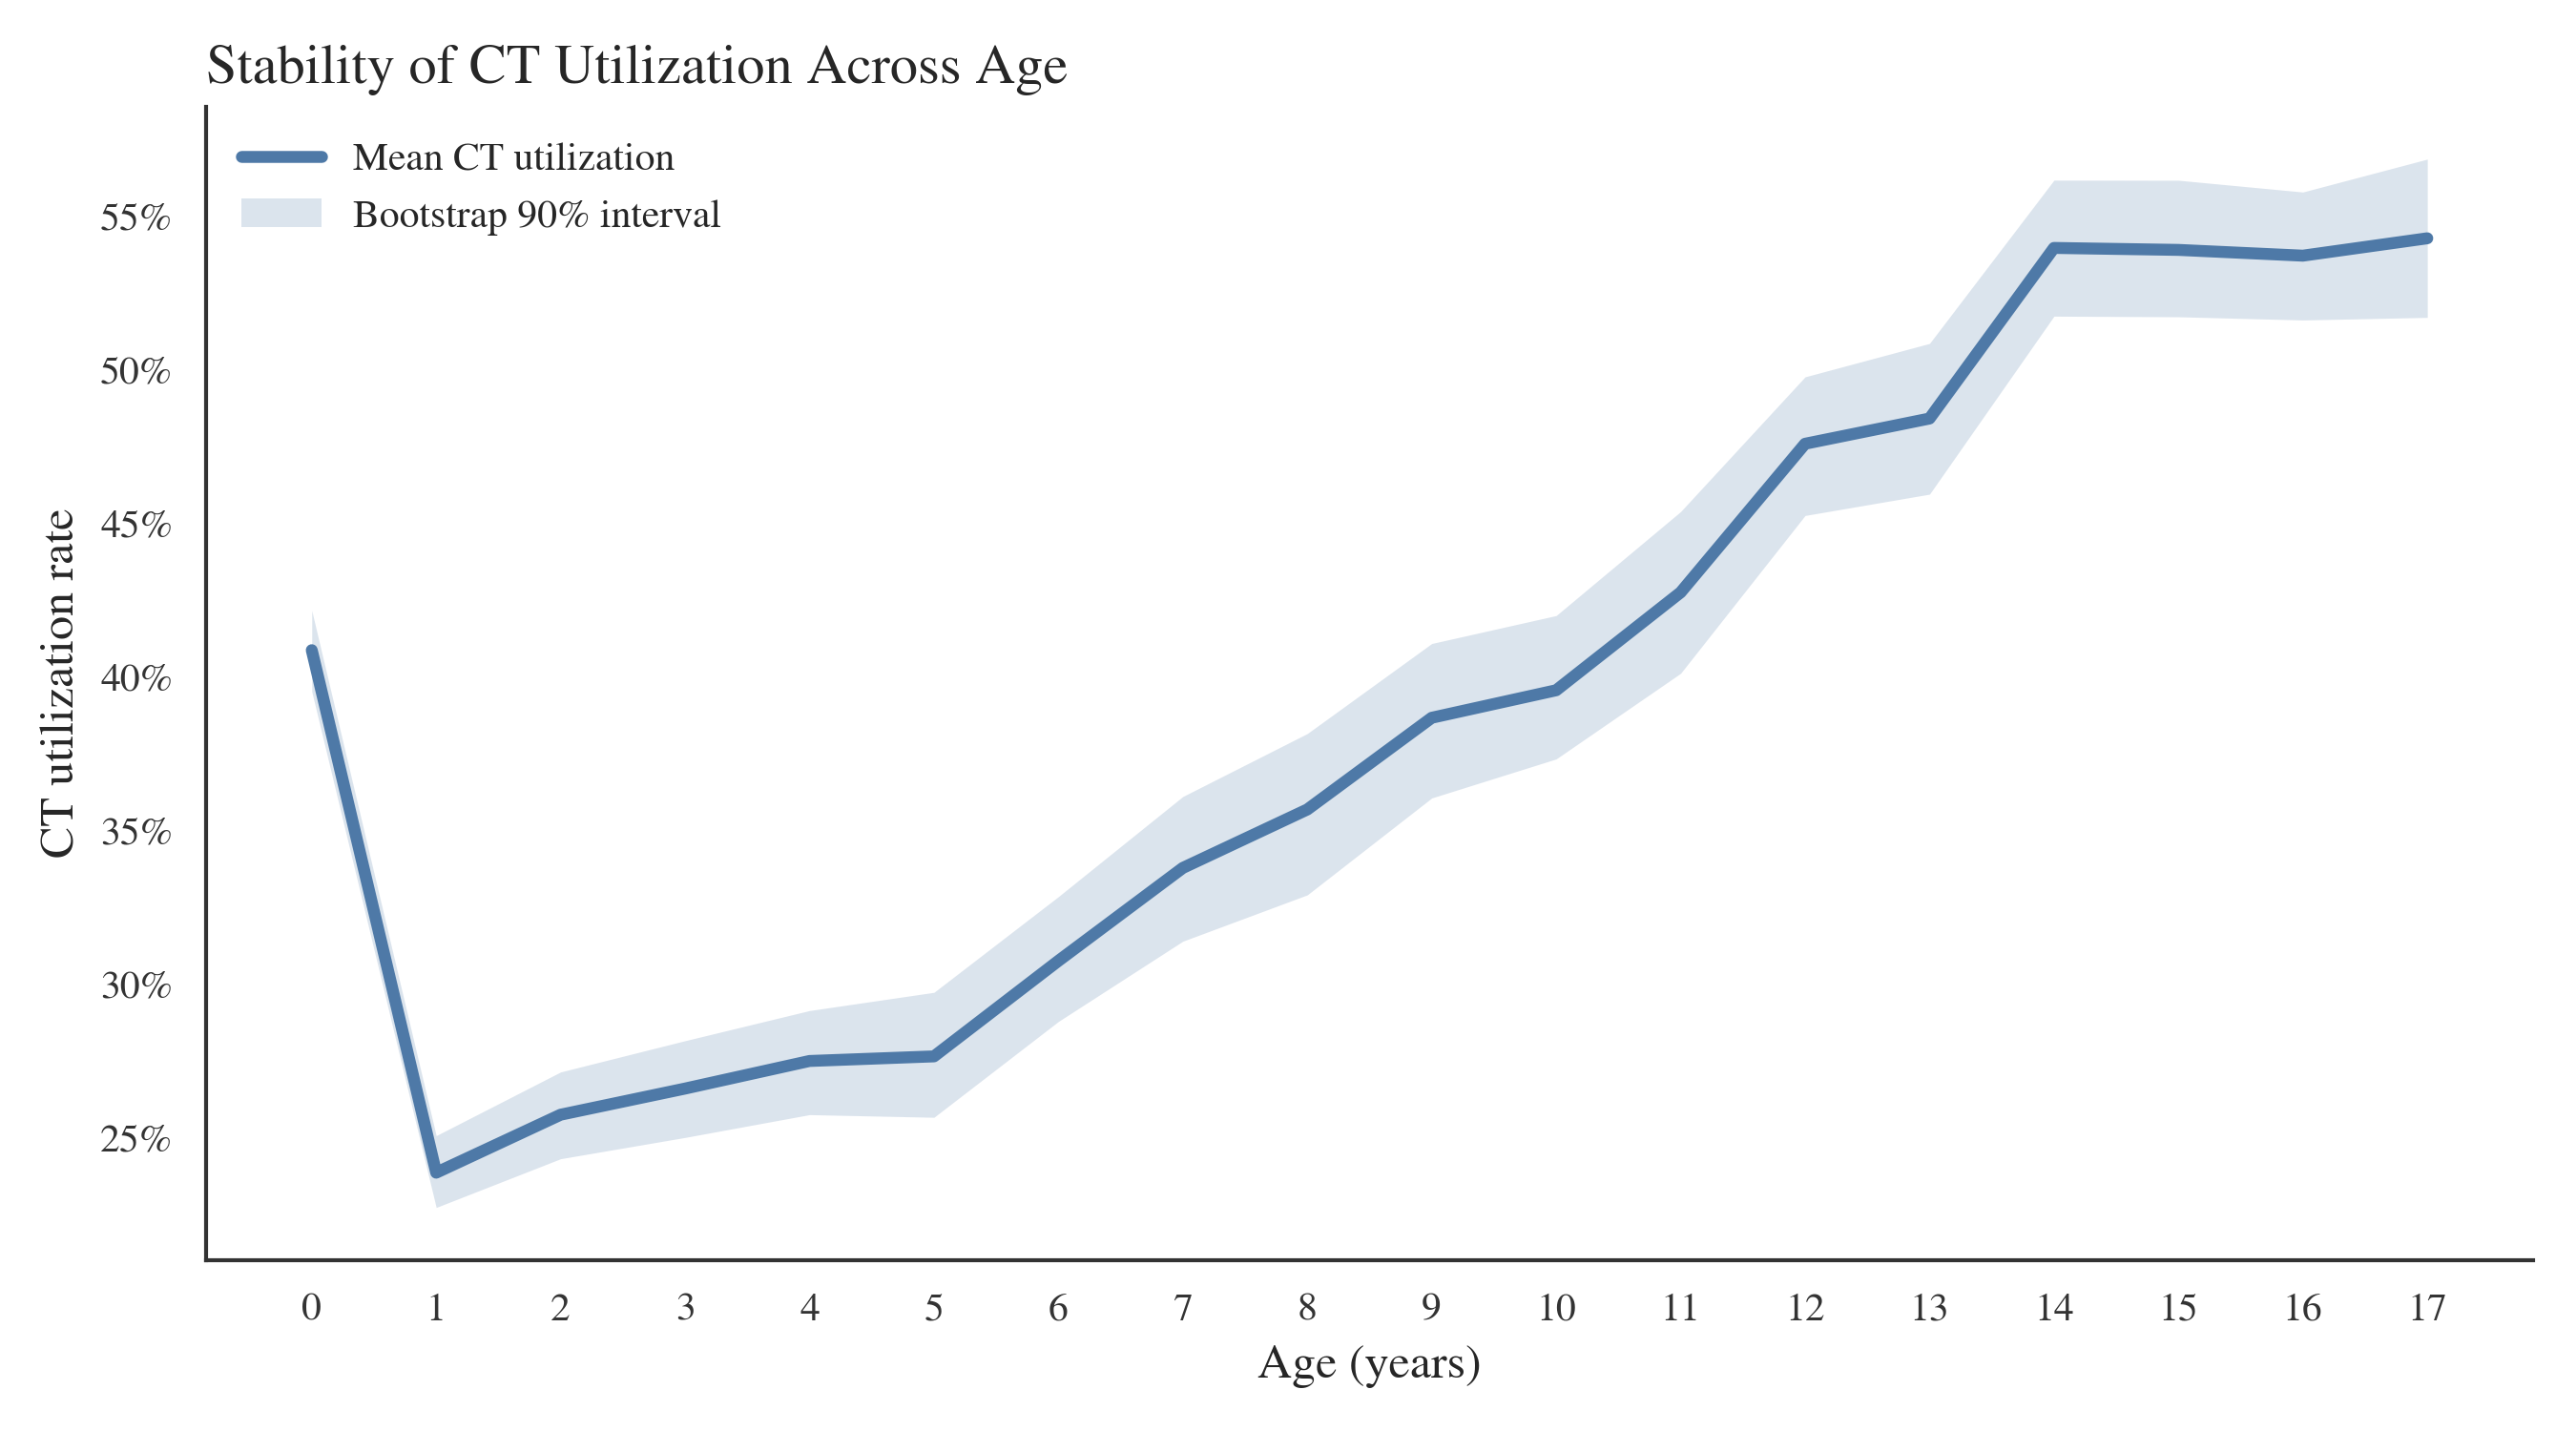
\includegraphics[
        height=0.25\textheight,
        width=\linewidth,
        keepaspectratio
        ]{../figs/ct_utilization_bootstrap.png}
    }
    \caption{Bootstrap: CT utilization curve shape is stable.}
    \end{subfigure}
    \caption{Robustness checks for the age-related CT imaging pattern. \textbf{Left}: small random perturbations to clinical indication variables. \textbf{Right}: bootstrap resampling confirms the CT utilization curve shape is stable.}
    \label{fig:age-stability}
\end{figure}


Actually, the stability check is not only for the first finding but also for all the findings in the data exploration section, referring to the related sections in \texttt{02\_eda.ipynb}. For example, for the second finding about the over-scan gap across mechanism, I also introduced bayesian inference to the observed risk and CT utilization for the tiny group with small sample size, and the pattern is still consistent with the original one.



\section{Modeling}

\subsection{Implementation}

\paragraph{Clinical Decision Rule (CDR).}
I implemented the original PECARN clinical decision rules as a baseline.
Following the original study, patients with GCS 3--13 were excluded and the rule was applied to classify patients into low- and high-risk groups. Model performance was evaluated using sensitivity and negative predictive value (NPV) across age groups and data splits.

\paragraph{Logistic Regression.}
Logistic regression serves as an interpretable benchmark capturing linear associations between predictors and ciTBI risk. Data preprocessing included missing indicators for binary variables, a ``missing'' category for multi-categorical features, imputation of GCS components, and one-hot encoding. Unlike the CDR, patients with GCS 3--13 were retained. Separate models were trained for the two age groups.

Feature selection combined simple screening (univariate association and near-constant features), LASSO regularization, and manual clinical filtering to reduce redundancy. Hyperparameters (regularization strength and class weights) were tuned using grid search for age $<2$ and random search for age $\geq2$, with model selection based on validation performance emphasizing Youden’s $J$ statistic.

\paragraph{CatBoost.}
CatBoost, a gradient boosting method designed for categorical data, was used as a nonlinear alternative. It directly handles categorical variables and missing values, eliminating the need for one-hot encoding. The same cohort (including GCS 3--13) and age-stratified modeling strategy were used.

Basic feature screening removed near-constant or weak predictors, while hyperparameters (learning rate, tree depth, and L2 regularization) were tuned via random search using validation performance balancing sensitivity and specificity. The key metric during training is the `PR-AUC` to account for class imbalance, while final evaluation focuses on sensitivity and NPV. 

The whole modeling process of data preparation, feature selection, training, hyperparameter tuning and evaluation is documented in \texttt{03\_prediction\_cdr.ipynb}, \texttt{04\_prediction\_lr.ipynb} and 

\texttt{05\_prediction\_catboost.ipynb} respectively. \texttt{models.py} contains the implementation of the three models and the evaluation function for reproducibility.

Table~\ref{tab:performance} summarizes model performance. All models achieve similar NPV ($\approx99\%$). As for the sensitivity, \textbf{CDR > CatBoost > Logistic Regression}. Compared with the CDR, logistic regression and CatBoost improve specificity but reduce sensitivity, reflecting a trade-off between avoiding missed cases and reducing unnecessary imaging. 

Moverover, during the training process, the logistic regression did \emph{not} converge for both groups, which may also contribute to the worse performance in sensitivity. 
Although I have adjusted the class weight to handle the imbalance, it may not be sufficient to make the model converge. For the two probability-based models, the choice of threshold also matters. I have tried different thresholds and the performance is not very stable, which may also contribute to the worse performance in sensitivity.

\renewcommand{\arraystretch}{0.85}
\begin{table}[htbp]
\centering
\small
\caption{Model performance across age groups and data splits.}
\label{tab:performance}
\begin{tabular}{llcccc}
\toprule
Model & Age group & Split & Sensitivity & Specificity & NPV \\
\midrule

\multirow{6}{*}{CDR}
& \multirow{3}{*}{Age $< 2$}
    & Train & 0.986 & 0.538 & 1.000 \\
&   & Val   & 1.000 & 0.544 & 1.000 \\
&   & Test  & 1.000 & 0.542 & 1.000 \\
\cmidrule(lr){2-6}
& \multirow{3}{*}{Age $\geq 2$}
    & Train & 0.969 & 0.575 & 1.000 \\
&   & Val   & 0.964 & 0.581 & 0.999 \\
&   & Test  & 0.964 & 0.583 & 0.999 \\

\midrule

\multirow{6}{*}{CatBoost}
& \multirow{3}{*}{Age $< 2$}
    & Train & 1.000 & 0.658 & 1.000 \\
&   & Val   & 0.933 & 0.690 & 0.999 \\
&   & Test  & 0.833 & 0.668 & 0.997 \\
\cmidrule(lr){2-6}
& \multirow{3}{*}{Age $\geq 2$}
    & Train & 0.981 & 0.757 & 1.000 \\
&   & Val   & 0.967 & 0.756 & 0.999 \\
&   & Test  & 0.984 & 0.760 & 1.000 \\

\midrule

\multirow{6}{*}{Logistic Regression}
& \multirow{3}{*}{Age $< 2$}
    & Train & 0.934 & 0.709 & 0.999 \\
&   & Val   & 1.000 & 0.723 & 1.000 \\
&   & Test  & 0.800 & 0.708 & 0.996 \\
\cmidrule(lr){2-6}
& \multirow{3}{*}{Age $\geq 2$}
    & Train & 0.729 & 0.927 & 0.995 \\
&   & Val   & 0.810 & 0.928 & 0.996 \\
&   & Test  & 0.769 & 0.933 & 0.995 \\

\bottomrule
\end{tabular}
\end{table}

\subsection{Interpretability}

The clinical decision rule is inherently interpretable since it is based on a set of explicit rules derived from clinical variables. Each rule corresponds to a specific clinical indication, making it straightforward to understand how the model arrives at its predictions.

Logistic regression is also interpretable, as the coefficients of the model indicate the direction and magnitude of the relationship between each predictor and the log-odds of the outcome. Catboost, on the other hand, is less interpretable due to its ensemble nature and complex interactions between features. However, we can still gain insights into feature importance.

To sum up, the CDR is the most interpretable model, followed by logistic regression, while CatBoost is the least interpretable. As for the specific features that are important in each model, beyond the original CDR variables, we find that some other predictors also have significant contributions to the model performance, such as \textbf{neurological deficit} and \textbf{seizure}. The importance of these features may vary across age groups, which is consistent with our earlier findings about age-related shifts in clinical decision drivers. Also, \textbf{missingness} indicators for certain variables also show up as important features, reinforcing the idea that missing data carries clinical signal in this dataset, which is aligned with my third finding.

\begin{figure}[htbp]
\centering

\begin{subfigure}{\textwidth}
    \centering
    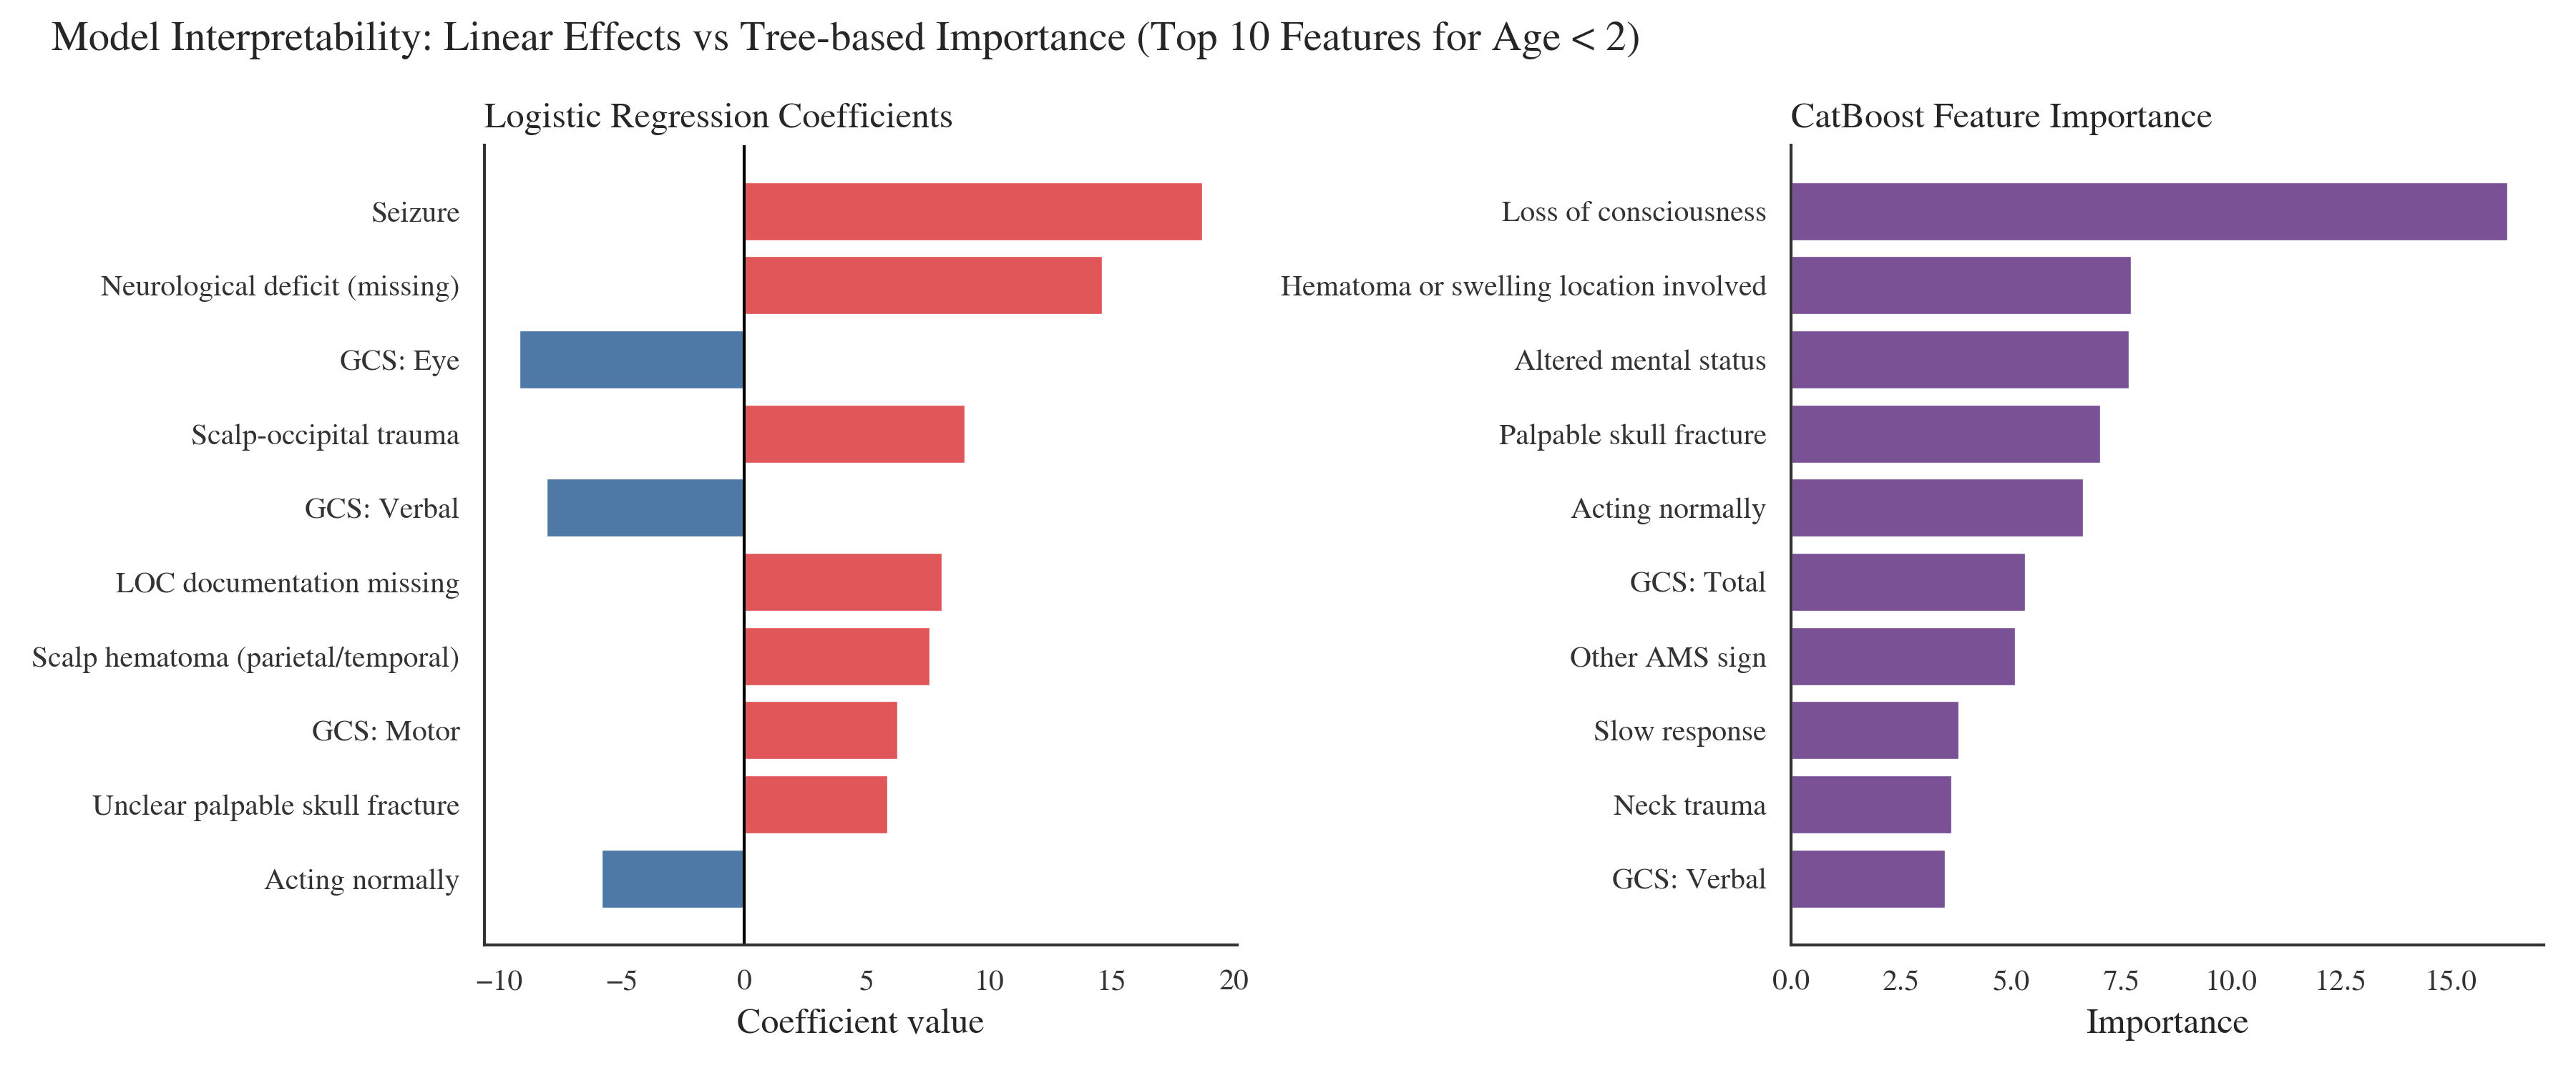
\includegraphics[width=\textwidth]
    {../figs/model_interpretability_age2mius.png}
    \caption{Age $<2$ years}
\end{subfigure}

\vspace{0.6em}

\begin{subfigure}{\textwidth}
    \centering
    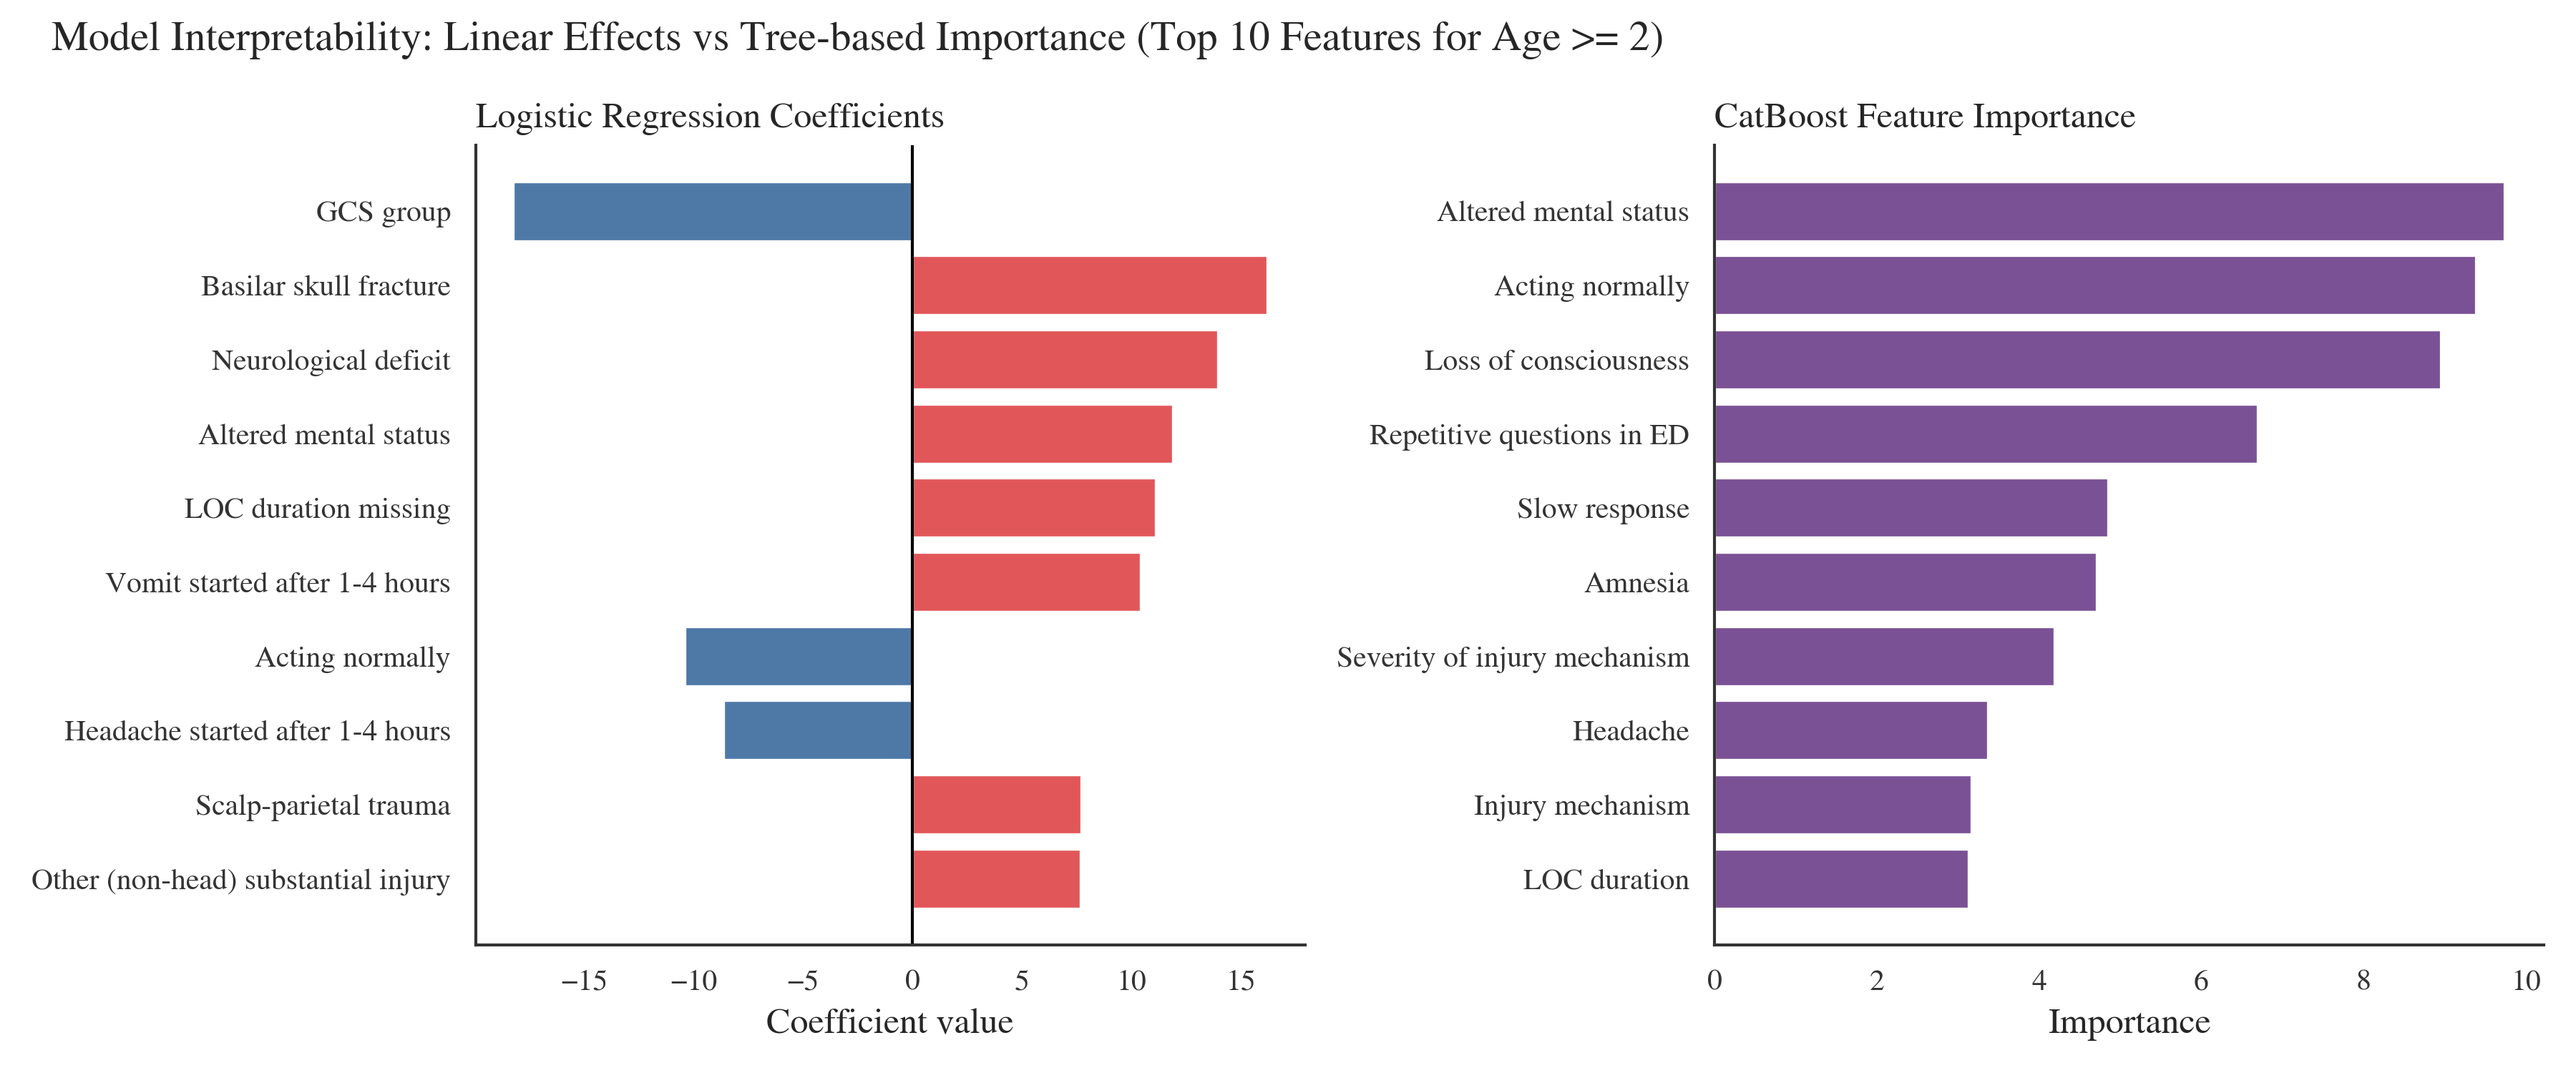
\includegraphics[width=\textwidth]
    {../figs/model_interpretability_age2plus.png}
    \caption{Age $\geq 2$ years}
\end{subfigure}

\caption{
Model interpretability comparison between logistic regression and CatBoost.
Left panels show standardized logistic regression coefficients, while right
panels show CatBoost feature importance rankings.
}
\label{fig:model-interpretability}
\end{figure}

\subsection{Stability}

For CDR model, I introduced small random perturbations to the core predictors (altered mental status, vomiting, basilar skull fracture and whether acting normally by parent) and evaluated how the performance metrics (sensitivity, specificity, NPV) changed across different age groups and data splits for CDR model. 

For logistic regression and CatBoost, I change one of the judgement calls in the data preprocessing stage, which is whether to impute missing GCS scores. I compare the performance metrics before and after this change across different age groups and data splits for both models. The reason behind this choice is that small random perturbations may not be enough to capture the stability of the model, since I include way more features than the original CDR, and the performance of the model may be more sensitive to the data preprocessing choices.

The results are summarized in Table~\ref{tab:stability}, where $\Delta$ represents the change in performance metrics after perturbation compared to the original performance. Overall, the changes in performance metrics are relatively small across all models and age groups, indicating that the models are stable and not overly sensitive to minor variations in the input data. 

The comparison of performance, interpretability and stability across the three models is documented in \texttt{06\_prediction\_comparison.ipynb}.

\renewcommand{\arraystretch}{0.85}
\begin{table}[htbp]
\centering
\small
\caption{Change in performance under data perturbation 
($\Delta$ = perturbed − original). Smaller absolute values indicate greater stability.}
\label{tab:stability}
\begin{tabular}{llcccc}
\toprule
Model & Age group & Split 
& $\Delta$ Sensitivity 
& $\Delta$ Specificity 
& $\Delta$ NPV \\
\midrule

\multirow{6}{*}{CDR}
& \multirow{3}{*}{Age $<$ 2}
    & Train & -0.001 & -0.048 &  0.000 \\
&   & Val   &  0.000 & -0.049 &  0.000 \\
&   & Test  & -0.002 & -0.048 &  0.000 \\
\cmidrule(lr){2-6} 
& \multirow{3}{*}{Age $\geq$ 2}
    & Train & -0.006 & -0.076 & -0.000 \\
&   & Val   &  0.003 & -0.075 &  0.000 \\
&   & Test  &  0.001 & -0.078 & -0.000 \\

\midrule

\multirow{6}{*}{CatBoost}
& \multirow{3}{*}{Age $<$ 2}
    & Train &  0.000 &  0.037 & 0.000 \\
&   & Val   &  0.067 &  0.025 & 0.001 \\
&   & Test  &  0.000 &  0.032 & 0.000 \\
\cmidrule(lr){2-6} 
& \multirow{3}{*}{Age $\geq$ 2}
    & Train &  0.002 &  0.005 & 0.000 \\
&   & Val   &  0.000 &  0.008 & 0.000 \\
&   & Test  & -0.008 &  0.005 & -0.000 \\

\midrule

\multirow{6}{*}{Logistic Regression}
& \multirow{3}{*}{Age $<$ 2}
    & Train & -0.012 &  0.032 & -0.000 \\
&   & Val   &  0.000 &  0.039 &  0.000 \\
&   & Test  & -0.033 &  0.041 & -0.001 \\
\cmidrule(lr){2-6} 
& \multirow{3}{*}{Age $\geq$ 2}
    & Train &  0.171 & -0.169 & 0.003 \\
&   & Val   &  0.065 & -0.161 & 0.001 \\
&   & Test  &  0.143 & -0.167 & 0.002 \\

\bottomrule
\end{tabular}
\end{table}


\section{Discussion}\label{discussion}

Although the PECARN dataset is large compared with previous studies which seldom include the pre-verbal patients, effective sample size varies across clinically meaningful subgroups. Rare clinical states and certain age–mechanism combinations contain few observations, leading to unstable empirical risk estimates. This created challenges during exploratory analysis, where small denominators sometimes produced extreme rates. To address this, subgroup sizes were reported explicitly and stability checks (perturbation and bootstrap) were used to verify the consistency.

This project can be viewed through three interacting realms. First, the data–reality realm includes cleaning and exploratory analysis, where clinical variables reflect both patient condition and physician documentation practices. Second, the algorithm–model realm includes clinical decision rule, logistic regression and CatBoost, which approximate patterns in the observed data under different modeling assumptions. Third, the future data–reality realm is addressed through robustness analyses, evaluating whether conclusions persist under resampling and small data changes.

There is not a one-to-one correspondence between data and reality. Clinical variables are filtered through measurement and decision processes; for example, missingness itself carried predictive signal, suggesting documentation behavior influences recorded data. Similarly, visualizations summarize complex uncertainty and may exaggerate patterns when subgroup sizes are small. Careful annotation and robustness checks were therefore necessary to ensure reliable interpretation.

Overall, consistent results across EDA, modeling, and stability analyses suggest that the observed age-related imaging patterns reflect a stable feature of clinical decision-making rather than an artifact of the dataset.

\section{Conclusion}\label{conclusion}


This project investigated the PECARN TBI dataset to better understand how CT imaging decisions relate to age, injury characteristics, and clinical documentation. Through careful data cleaning and exploratory analysis, three consistent patterns emerged: \textbf{CT utilization varies non-monotonically with age}, \textbf{imaging behavior differs across injury mechanisms}, and \textbf{missing clinical variables themselves carry predictive signal}. Together, these findings suggest that imaging decisions are influenced not only by observed injury risk but also by diagnostic uncertainty and clinical workflow.

Modeling results showed that while machine learning approaches (logistic regression and CatBoost) improve specificity compared with the original clinical decision rule (CDR), they do so at the cost of reduced sensitivity. Given the clinical priority of avoiding missed ciTBI cases, this highlights an inherent trade-off between reducing unnecessary imaging and maintaining patient safety. Interpretability analyses further demonstrated that important predictors align with clinical reasoning, including neurological status, loss of consciousness, and behavioral abnormalities, while missingness indicators captured latent physician decision processes.

Reality and stability checks confirmed that the observed patterns are robust to preprocessing choices, perturbations, and resampling. Overall, the results indicate that age-dependent imaging behavior is a stable feature of clinical decision-making rather than a statistical artifact. The analysis reinforces the value of combining interpretable clinical rules with data-driven modeling while recognizing that medical data reflect both patient physiology and human decision processes.

\section{Academic honesty statement}\label{academic-honesty-statement}

Dear Bin,

I certify that this work is my own and that all sources and discussions have been properly cited. Academic honesty is necessary to ensure transparency, reproducibility, and trust in scientific research.

\section{Collaborators}\label{collaborators}
Since this is an individual project, I did not have any collaborators. However, I did have discussions with Bin about the missingness handling strategy, which helped me to clarify my thinking and improve my analysis. 
\renewcommand{\refname}{}
\section{Bibliography}\label{bibliography}

\begin{thebibliography}{9}
\setlength{\itemsep}{0pt}  % optional: tighter spacing

\bibitem{Kuppermann2009}
N.~Kuppermann, J.~F. Holmes, P.~S. Dayan, et al.
Identification of children at very low risk of clinically-important brain injuries after head trauma:
a prospective cohort study.
\textit{The Lancet}, 374(9696):1160--1170, 2009.

\end{thebibliography}
\end{document}

